\chapter{多终端协同服务任务调度算法}\label{chap:task_scheduling}

\section{引言}

任务调度问题是指系统在同时接收到多个服务请求任务的时候,将这些任务合理地分配给多个智能终端上的容器进行处理,由于不同的容器所在智能终端的处理能力不同,每个容器所占用的资源也不同,导致不同的调度方案结果会有差异,需要针对在容器化智能终端协同服务场景下的一些特点来进行取舍和进一步的优化,以追求对于终端资源利用的最大化。在该任务场景下,最常见的用户需求就是实时性需求,也即要求任务能够被快速响应、快速执行、且执行结果能够快速回传给用户,因此最小化任务完成时间是任务调度问题最主要的目标。除此之外,需要考虑的因素还涉及硬件设备功耗、分布式设备负载均衡度等。

本章的内容组织结构如下:第\ref{sec:task_scheduling_related_work}节介绍了任务调度问题算法的相关研究工作,包括传统的基于局部贪心策略的任务调度算法以及基于元启发式算法的任务调度算法;第\ref{sec:task_scheduling_GOA}节介绍了蝗虫优化算法(GOA)的背景、原理、数学模型以及数学表达式;第\ref{sec:task_scheduling_DJGOA}节提出了一种带随机跳出机制的动态权重蝗虫优化算法(DJGOA),介绍了其随机跳出机制以及动态权重策略,列出了所提出的带随机跳出机制的动态权重蝗虫优化算法在测试函数上的测试结果,并根据测试结果对带随机跳出机制的动态权重蝗虫优化算法的性能进行了分析;第\ref{sec:task_scheduling_IGOA}节在第\ref{sec:task_scheduling_DJGOA}节提出的算法的基础上,进一步提出了一种改进蝗虫优化算法(IGOA),介绍了其非线性舒适区控制参数、基于$L\acute{e}vy$飞行的局部搜索机制以及基于线性递减参数的随机跳出策略,列出了所提出的改进蝗虫优化算法在测试函数上的测试结果,并根据测试结果对改进蝗虫优化算法的性能进行了分析;第\ref{sec:task_scheduling_problems}节介绍了任务调度问题,提出了多终端协同服务环境中的任务调度问题的数学模型,并将第\ref{sec:task_scheduling_IGOA}节所提出的改进蝗虫优化算法应用到该模型中来求最优解,进行了仿真实验并分析实验结果;第\ref{sec:task_scheduling_summary}节对本章内容进行了总结。

\section{相关工作}\label{sec:task_scheduling_related_work}

\subsection{传统任务调度问题求解方法}

任务调度问题是将多个任务计划到约束下的多个节点的问题。任务调度问题是一个优化问题,任务调度问题也是一个NP-hard问题\cite{tawfeek2013cloud},已有的任务调度算法主要分为两大类,一类是基于局部贪心策略的算法,另一类是启发式的智能搜索方法。有很多传统的基于贪心策略的任务调度优化算法\cite{乔楠楠2017一种面向网络边缘任务调度问题的多方向粒子群优化算法}。先进先出算法(FIFO Scheduler)是按照任务到达的先后顺序进行调度\cite{zaharia2009job},Max-Min算法是优先调度执行时间最长的任务,Min-Min算法是优先调度执行时间最短的任务,\cite{tabak2014improving,杜玉霞2010Min}。这些基于贪心策略的任务调度算法的优点是原理比较简单,方便实施,运行速度快。但同样是因为这些算法的原理过于简单,优先满足局部最优选择,导致其缺点是很容易陷入局部最优解,得不到效果更好的解决方案。尤其是当任务规模扩大的时候,任务的维度也会增加,这会扩大搜索空间并使优化问题更加复杂,基于贪心策略的传统任务调度算法无法处理这种情况。

% 任务调度问题是将多个任务计划到约束下的多个节点的问题。任务调度问题是一个优化问题。应用多种算法来解决任务调度问题。基于最佳资源选择 (BRS) 的算法, 如最大最小、最小、苦难等, 是解决任务调度问题的传统方法。一些元启发式算法, 如 PSO 和基于 pso 的改进算法, 是处理任务调度问题的新方法。

\subsection{启发式算法求解方法}
% 启发式算法则是确定搜索策略,通过迭代、评价等方式,逐步逼近全局最优解。

近年来, 学者们对任务调度问题进行了大量的研究。随着研究的进行, 许多元启发式算法(Meta-Heuristic Algorithm)被用来处理复杂的优化问题。元启发式算法具有操作简单和开销较少的优点, 能够在最优化问题(Optimization Problem)中找到全局最优解或近似全局最优解。

Goldberg于1988年提出了遗传算法(Genetic Algorithm, GA)\cite{fonseca1995overview,whitley1994genetic,tanese1989distributed,Nagham2018}。遗传算法是一种经典的元启发是算法,将自然选择理论引入到寻优的过程中,算法模拟了达尔文生物进化论中的包含自然选择和遗传机制的生物进化过程的计算模型,通过模拟自然进化的过程来搜索问题空间内的最优解。遗传算法用一个染色体来表示一种可行的解,并利用交叉、变异、选择等运算符实现可行解的进化,经过若干轮的不断迭代和演进,最终得到比较好的全局最优解或近似最优解。虽然遗传算法的性能非常好, 但是遗传算法的操作比较复杂,运算量较大,收敛速度较慢,不适合应用于多终端协同任务调度问题的求解。Kirkpatrick于1983年提出模拟退火算法(Simulated Annealing Algorithm,SA),是一种基于概率的算法。模拟退火算法模拟固体退火过程,从某一较高初温出发,随着温度参数的不断下降,动态调整跳出的概率,在解空间中随机寻找目标函数的全局最优解,即在局部最优解中以一种动态的概率进行跳出并最终趋于全局最优\cite{kirkpatrick1983optimization,Hong1991A,rutenbar1989simulated}。但尽管如此,模拟退火算法还是很容易陷入局部最优。

一些元启发式算法的灵感来自昆虫、鱼类、鸟类和其他群体生物的自然行为。Kennedy和Eberhart在1995年提出粒子群算法(Particle Swarm Optimization, PSO),是一种非常经典的元启发式算法\cite{kennedy1995particle,liao2007discrete,krishnasamy2013task}。该算法最初是受到飞鸟集群活动的规律性启发,利用群体智慧建立的一个简化模型,通过追随当前搜索到的最优值来寻找全局最优。粒子群算法的原理简单,易于实现,而且性能非常好。蚁群优化算法(Ant Colony Optimization Algorithm, ACO)是受蚂蚁在蚁巢和食物来源之间自然觅食行为的启发而提出的一种算法\cite{dorigo1997ant,dorigo1999ant,郝航2018基于并行化蚁群算法的网络测量节点选取算法}。蚁群算法利用化学信息素在蚂蚁群之间进行通信和交换信息,以控制整个蚁群的搜索方向。布谷鸟算法(Cuckoo Search Algorithm, CS)是Yang在2009年提出的一种元启发式算法\cite{yang2009cuckoo}。布谷鸟算法的灵感来自布谷鸟的繁殖行为,该算法使用$L\acute{e}vy$飞行来跳出局部最优。

Some novel meta-heuristic optimization algorithms are proposed recently. There are not many pieces of research on the improvement of those algorithms. The Ant Lion Optimizer proposed in 2015 is inspired by the hunting behavior of antlions \cite{mirjalili2015ant}. Whale Optimization Algorithm (WOA) was proposed in 2016. WOA simulates the natural hunting behavior of whales \cite{mirjalili2016WOA}. Dragonfly Algorithm (DA) proposed in 2016 is inspired by the static and dynamic behaviors of the dragonfly swarm in nature \cite{mirjalili2016dragonfly}. In 2017, Shahrzad Saremi and Seyedali Mirjalili proposed a novel meta-heuristic optimization algorithm called Grasshopper Optimization Algorithm (GOA). GOA simulates the migration behavior of the grasshopper swarm by utilizing the influence of the interaction within the swarm and the wind influence outside the swarm to find the target food \cite{saremi2017grasshopper}. 

最近提出了一些新的元启发式优化算法。关于改进这些算法的研究并不多。蚂蚁狮子优化器提出 (ALO) 在2015年是受狮子 \ citemirjilili2013 蚂蚁的狩猎行为的启发。鲸鱼优化算法 (WOA) 于2016年提出。WA 模拟鲸鱼的自然狩猎行为。2016年提出的蜻蜓算法 (DA) 是受蜻蜓群在自然界中的静态和动态行为的启发。


2017年, Shahrzad Saremi 和 Seyedali Mirjalili 提出了一种新的元启发式优化算法, 称为蝗虫优化算法 (GOA)。GOA 利用群体内部的相互作用和蜂群外的风的影响来模拟蝗虫群的迁徙行为, 寻找目标食物 \ citesare2013 2017 蝗虫。GOA 算法利用群智能, 通过在蝗虫群之间分享经验, 确定搜索方向, 找到最佳或近似的最佳位置。GOA 还使用了具有多个迭代的进化方法, 以提高群智能的效率。

GOA has been widely used in many areas since it was proposed. S.~Łukasik used GOA to generate accurate data clusterings and compare the performance with the standard K-means algorithm \cite{Łukasik}. Neelam Rajput applied GOA to solve 3 types of economic dispatch problems in electrical power systems, and the results of the experiments showed that GOA is superior to other methods\cite{rajput}. Zahra Elmi employed GOA to search for a better path in robot navigation \cite{elmi}. Deepak Kumar Lal used GOA to tune controller gains in Fuzzy PID controller \cite{lal}. Some other literature can also show that GOA is competitive in many research and practice fields \cite{hamour,hekimoglu,ahanch,amaireh,barik}. 

开发了一些基于 GOA 的改进算法。OBLGOA 是由艾哈迈德·埃维斯在2018年提出的 \ ceewees 2013 改进。根据目前的搜索位置, 引入了基于对立面的学习策略, 以生成相反的解作为候选方案。OBL 策略可以提高算法的收敛速度, 但由于缺乏随机性, 改进有限。桑卡拉阿罗拉提出了混沌蝗虫优化算法在 2018年 \ 柠檬酸乱糟糟。将混沌映射应用到算法中, 提高了 GOA 的性能。采用10幅混沌映射来评价混沌理论的影响。结果并不是特别理想, 因为混沌因素在处理许多基准函数时并不合适。提出了一种基于 GOA 的新算法来解决优化问题和任务调度问题。

\section{GOA算法}\label{sec:task_scheduling_GOA}
\subsection{GOA算法背景}
\subsection{GOA算法数学模型}
蝗虫优化算法模拟蝗虫的昆虫群行为。蝗虫蜂拥而至, 远距离迁徙, 寻找一个有食物的新栖息地。在这个过程中, 蝗虫之间的互动在蜂群内部互相影响。风的力量和蜂群外的重力影响蝗虫的轨迹。食物的目标也是一个重要的影响因素。

受上述三个因素的影响, 移民过程分为勘探和开发两个阶段。在勘探阶段, 鼓励蝗虫快速、突然地移动, 寻找更多潜在的目标区域。在开发阶段, 蝗虫往往在当地移动, 以寻找更好的目标地区。蝗虫自然实现了勘探开发寻找食物来源的两种迁徙趋势。此过程可以抽象为优化问题。蝗虫群被抽象为一群搜索代理。

Seyedali Mirjalili 在文献[]中提出了蝗虫群体迁移的数学模型。具体的模拟公式如下:

\begin{equation}
    X_i = S_i + G_i + A_i 
\end{equation}

这里变量$X_i$是第i个搜索单位的位置,变量$S_i$代表蝗虫集群内部搜索单位间社会交互对第i个搜索单位的影响因子,变量$G_i$代表蝗虫集群外部重力因素对第i个搜索单位的影响因子,变量$A_i$代表风力的影响因子。变量$S_i$的定义公式如下:

\begin{equation}
    S_i = \sum_{j=1, j\neq{i}}^N s(d_{ij})\widehat{d_{ij}}
\end{equation}

这里变量$d_{ij}$代表第i个搜索单位和第j个搜索单位之间的欧式距离,计算方法如下:
\begin{equation}
    d_{ij}=|x_j-x_i|
\end{equation}

变量$\widehat{d_{ij}}$代表第i个搜索单位和第j个搜索单位之间的单位向量,计算方法如下:

\begin{equation}
    \widehat{d_{ij}}=\frac{x_j-x_i}{d_{ij}}
\end{equation}

\emph{s}是一个函数,用于计算蝗虫集群之间的社会关系影响因子,该函数定义如下:

\begin{equation}
    s(r) = fe^{\frac{-r}{l}}-e^{-r}
\end{equation}

这里\emph{e}是自然底数,变量\emph{f}代表吸引力因子,参数\emph{l}代表吸引力长度。
% where \emph{e} is the Natural Logarithm, \emph{f} represents the concentration of attraction and the parameter of \emph{l} shows the attractive length scale.
当应用于解决数学优化问题的时候,为了优化数学模型,公式1中需要加入一些适当的改动。代表集群外部影响因子的变量$G_i$和$A_i$需要被替换为目标食物的位置。这样计算公式就变成了如下的样子:

\begin{equation}
    x_i = c \Bigl(\sum_{j=1,j\neq{i}}^N c \frac{u-l}{2}s (\lvert x_j-x_i \rvert )\frac{x_j-x_i}{d_{ij}} \Bigr) + \widehat{T_d}
\end{equation}

这里参数\emph{u}和参数\emph{l}分别代表搜索空间的上界和下界。变量$\widehat{T_d}$是目标食物的位置,在优化问题的数学模型中代表所有搜索单位在整个搜索过程中所能找到的最优的解的位置。另外,参数\emph{c}是搜索单元的搜索舒适区控制参数,改变参数\emph{c}的大小可以平衡搜索过程中的“开拓”和“探索”两个阶段。参数\emph{c}的计算方式如下:

\begin{equation}
    c = cmax - iter \frac{cmax - cmin}{MaxIteration}
\end{equation}


这里参数\emph{cmax}和参数\emph{cmin}分别是参数\emph{c}的最大值和最小值,参数\emph{iter}代表当前的迭代次数,参数\emph{MaxIteration}代表最大迭代次数。

在优化问题的求解过程中,公式4作为演进公式,被不断循环迭代来寻找最优解,直到达到迭代终止条件为止。通常迭代终止条件为达到预设的最大迭代次数,或者所得到的最优解满足预设的最优解条件。在本研究所涉及到的优化问题中,迭代终止条件均为达到预设的最大迭代次数。在迭代演进的过程结束后,该算法可以得到一个近似的最优解的位置以及相应的最优解的值。

蝗虫优化算法的算法伪代码如\ref{alg:GOA}所示:
\begin{algorithm}
    % \setstretch{1.35}

    \caption{蝗虫优化算法}
    \label{alg:GOA}
    
    \begin{algorithmic}[1]
    \State initialize the swarm and set the position boundaries u and l
    \State initialize the factors including cmax, cmin, MaxIteration
    \State initialize all the search agents position with random origin matrix 
    \State calculate the target fitness and mark the target position
    
    \While {$(iter < MaxIteration$ and $target fitness > destination fitness)$}
    \State calculate $d_ij$ and $\widehat{d_ij}$ by equation(2)
    \State calculate $s(d_ij)$ by equation(3)
    \State update $x_i$ by equation(4)
    \State calculate the fitness 
    \If{current fitness is better than target fitness}
        \State update the target fitness and the target position
    \EndIf
    \State $iter = iter +1$
     
    \EndWhile

    \State Return target fitness and target position
    
    
    \end{algorithmic}
    
\end{algorithm}

\subsection{蝗虫算法优缺点分析}
GOA是最近受到蚱蜢自然迁移行为启发的元启发式算法。 虽然GOA具有简单的理论基础并且易于实现,但GOA的性能更优越。 原始的GOA改变了蚱蜢的舒适区域,这可以使目标通过迭代收敛到全局最优解。 与一些经典算法相比,GOA的收敛速度要快得多。 GOA可显着提高蝗虫的平均适应度,改善蝗虫的初始随机种群。虽然GOA具有这些优点,但它也存在一些阻碍算法获得更好解决方案的缺点。 在对GOA公式进行一些理论分析和用MATLAB代码进行的一些实验之后,给出了GOA的几个缺点。

首先,GOA使用线性递减参数使搜索过程收敛,这很难区分过程的两个阶段,即开发阶段和探索阶段。 其次,在搜索过程的早期阶段的每次迭代期间,最佳解决方案的位置急剧波动。 似乎最终的最佳解决方案只受搜索过程后期的影响,无论前一阶段的结果如何。 GOA理论无法充分利用所有搜索迭代。 当最大迭代次数增加时,GOA的最佳适应性不是很突出,例如,从实验结果中发现的500到1500。 最后,搜索过程很容易陷入局部最优。 GOA易于实现的优势无助于摆脱局部最优,这可能是GOA的劣势。


\section{带随机跳出机制的动态权重蝗虫优化算法(DJGOA)}\label{sec:task_scheduling_DJGOA}
\subsection{动态权重}
GOA使用线性递减参数来限制搜索空间并使所有搜索代理移动到目标位置。 线性递减参数不能增强搜索过程的两个阶段的影响,即开发阶段和探索阶段。 在探索阶段,GOA无法在目标搜索区域周围快速收敛,搜索代理只是在整个搜索空间中游荡,这无法为后期搜索阶段奠定坚实的基础。 在开发阶段,参数通常使搜索代理滑过局部最佳位置,就像搜索代理超速运动一样。

线性递减参数机制无法使算法充分利用整个迭代。 引入动态权重参数机制以提高算法的利用率。 搜索进度分为三个阶段,即早期阶段,中间阶段阶段和后期阶段。 在早期阶段,目标位置的权重应该更高,以使搜索过程快速收敛。 在中间阶段,参数应该是稳定的,以使算法探索搜索空间。 在后期阶段,搜索代理中的重力的权重应该更小,以深入利用局部最优解位置。 具有动态权重参数的GOA公式表示为算法[1]。 新的迭代方程如下:

\begin{equation}
    x_i = m*c \Bigl(\sum_{j=1,j\neq{i}}^N c \frac{u-l}{2}s (\lvert x_j-x_i \rvert )\frac{x_j-x_i}{d_{ij}} \Bigr) + \widehat{T_d}
\end{equation}
where \emph{m} is the dynamic weight parameter to adjust the search process. To correspond to the feature of the three phases of the search process, the parameter \emph{m} is set as follows:
\begin{equation}
    m= \begin{cases}
        0.5-\frac{(0.5-0.1)*iter}{MaxIteration*0.2} & \quad 0<iter\leq MaxIteration*0.2 \\
        0.1&\quad MaxIteration*0.2<iter \leq MaxIteration*0.8 \\
        0.05& \quad  MaxIteration*0.8 < iter \leq MaxIteration
        \end{cases} 
\end{equation}

\subsection{随机跳出机制}

原始的GOA算法没有使用跳跃机制,并且所有搜索代理仅根据社交互动和目标食物吸引力的影响而移动。 原始GOA的机制可能导致算法陷入局部最优位置。

引入随机跳跃策略以帮助GOA算法提高跳出局部最佳位置的概率。 参数\emph{p}被设置为跳跃阈值。 在迭代结束之前,将当前最佳适合度与最后一次迭代的最佳适应度进行比较。 如果当前最佳适应度和最后一个最佳适应度的比率高于阈值\emph{p},则可以假设该算法没有找到更好的解决方案,并且随机跳跃机制应该启动。 根据随机初始化规则在最佳位置周围生成新的搜索代理。 随机初始化规则如下:
\begin{equation}
    tempPos=curPos*((0.5-rand)*iniRan+1);
\end{equation} 
其中\emph{tempPos}是新搜索代理的位置,\emph{curPos}是当前最佳解决方案的位置。 \emph{iniRan}是管理随机跳跃边界的初始化范围参数。 如果\emph{iniRan}更高,则算法的全局搜索能力就像模拟退火算法一样得到增强。
\subsection{DJGOA算法流程}

本文提出了一种随机跳跃动态权重蝗虫优化算法(DJGOA)。 DJGOA的过程分为初始阶段,参数设置阶段,计算阶段和适应度更新阶段四个阶段。在初始化阶段,设置包括位置边界在内的一些因素,并在边界内随机初始化原始群体位置。在参数设置阶段,搜索过程进入迭代循环,动态权重参数根据当前迭代由\ emph {equation(7)}设置。在计算阶段,群体内的社会交互由\ emph {equation(6)}计算。在适应度更新阶段,如果当前适应度优于历史的最佳目标适应度,则更新目标解决方案的适合度。如果当前适应度与最后一次迭代的适应度之比高于之前设置的阈值\ emph {p},则使用随机跳转策略生成新的搜索代理以尝试跳出局部最优位置通过\ emph {equation(8)}。具有随机跳跃的动态权重蝗虫优化算法(DJGOA)的伪代码显示为算法\ref{alg:DJGOA}。

\begin{algorithm}
    % \setstretch{1.35}

    \caption{带随机跳出机制的动态权重蝗虫优化算法}
    \label{alg:DJGOA}
    
    \begin{algorithmic}[1]
    
    \State initialize the swarm and set the position boundaries u and l
    \State initialize the factors including cmax, cmin, MaxIteration and iniRan
    \State initialize all the search agents position with random origin matrix 
    \State calculate the target fitness and mark the target position
    
    \While {$(iter < MaxIteration$ and $target fitness > destination fitness)$}
    \State set the dynamic weight parameter m by equation(7)
    \State calculate $d_ij$ and $\widehat{d_ij}$ by equation(2)
    \State calculate $s(d_ij)$ by equation(3)
    \State update $x_i$ by equation(6)
    \State calculate the fitness 
    \If{current fitness is better than target fitness}
        \State update the target fitness and the target position
    \EndIf
    \If{$(current fitness/last fitness) > p$}
        \State generate a new search agent by equation (8)
        \If{the new fitness is better than target fitness}
            \State update the target fitness and the target position
        \EndIf
    \EndIf
     
    \EndWhile

    \State Return target fitness and target position
    
    
    \end{algorithmic}
    
\end{algorithm}

\subsection{实验结果}
\subsubsection{实验设置}

为了评估所提算法的性能,进行了一系列实验。 我们将所提出的DJGOA与GOA的原始算法(最近的Dragonfly算法(DA)的元启发式算法)和粒子群算法(PSO)的经典启发式算法进行了比较,该算法通过在\ cite {saremi2017grasshopper}中使用的13个基准函数。 13个基准功能分为两种类型。 函数\ emph {f1-f7}是单峰函数,它测试了算法的收敛速度和局部搜索能力。 函数\ emph {f8-f13}是多模函数,当存在多个局部最优时,它测试算法的全局搜索能力。 表\ref{tab:unimodal_function}中列出了7个单峰测试函数的详细信息和表达式,表\ref{tab:multimodal_function}中列出了6个多峰测试函数的详细信息和表达式。
\begin{table}[!htbp]
    \centering
    \caption{F1-F7单峰测试函数}
    \label{tab:unimodal_function}
    % \small
    \renewcommand\arraystretch{1.5} 
\begin{tabular}{l c c c}
  \hline
  Function & Dim & Range & $f_{min}$ \\
  \hline
  $F_1(x)=\sum_{i=1}^n x_i^2$ & 30 & [-100,100]&0 \\
  \hline
  $F_2(x)=\sum_{i=1}^n\left|x_i\right|+\prod_{i=1}^n\left|x_i\right|$& 30 & [-10,10]&0 \\
  \hline
  $F_3(x)=\sum_{i=1}^n(\sum_{j=1}^ix_j)^2$& 30 & [-100,100] & 0\\
  \hline
  $F_4(x)=max_i\{\left|x_i\right|,1\leq i\leq n\}$& 30 & [-100,100] & 0\\
  \hline
  $F_5(x)=\sum_{i=1}^{n-1}[100(x_{i+1}-x_i^2)^2+(x_i-1)^2]$& 30 & [-30,30] & 0\\
  \hline
  $F_6(x)=\sum_{i=1}^n([x_i+0.5])^2$& 30 & [-100,100] & 0\\
  \hline
  $F_7(x)=\sum_{i=1}^n ix_i^4 + random[0,1)$& 30 & [-1.28,1.28] & 0\\
  \hline
\end{tabular}
\end{table}


\begin{table}[!htbp]
    \centering
    \caption{F8-F13多峰测试函数}
    \label{tab:multimodal_function}
    \small
    \renewcommand\arraystretch{1.5} 
\newcommand{\tabincell}[2]{\begin{tabular}{@{}#1@{}}#2\end{tabular}}
\begin{tabular}{l c c c}
    \hline
    % after \\: \hline or \cline{col1-col2} \cline{col3-col4} ...
    Function & Dim & Range & $f_{min}$ \\
    \hline
    $F_8(x)=\sum_{i=1}^n -x_i \sin(\sqrt{|x_i|})$ & 30 & [-500,500]&$-418\times Dim$ \\
    \hline
    $F_9(x)=\sum_{i=1}^n [x_i^2 - 10\cos(2\pi x_i)+10]$& 30 & [-5.12,5.12]&0 \\
    \hline
    % $F_{10}(x)=-20exp(-0.2\sqrt{\frac{1}{n}\sum _{i=1}^n x_i^2})-exp(\frac{1}{n}\sum_{i=1}^n \cos(2\pi x_i))+20+e$& 30 & [-32,32] & 0\\
    % \hline
    \tabincell{c}{$F_{10}(x)=-20exp(-0.2\sqrt{\frac{1}{n}\sum _{i=1}^n x_i^2})-$\\$exp(\frac{1}{n}\sum_{i=1}^n \cos(2\pi x_i))+20+e$}& 30 & [-32,32] & 0\\
    \hline
    $F_{11}(x)=\frac{1}{4000}\sum_{i=1}^n x_i^2 - \prod_{i=1}^n \cos(\frac{x_i}{\sqrt{i}})+1$& 30 & [-600,600] & 0\\
    \hline

    \tabincell{c}{$F_{12}(x)=\frac{\pi}{n} \{10\sin(\pi y_1)+\sum_{i=1}^{n-1} (y_i-1)^2 [1+10 \sin^2 (\pi y_{i+1} )]+ $ \\ $(y_n -1)^2\}+ \sum_{i-1}^n u(x_i,10,100,4)+\sum_{i=1}^n u(x_i,10,100,4)$\\ $y_i=1+\frac{x_i+1}{4}$ \\$u({x_i},a,k,m) = \left\{ \begin{array}{l}k{({x_i} - a)^m}{\rm{   }}{x_i} > a\\0{\rm{                }} - a < {x_i} < a\\k{( - {x_i} - a)^m}{\rm{  }}{x_i} <  - a\end{array} \right.$ }& 30 & [-50,50] & 0\\
    \hline
    \tabincell{c}{$F_{13}(x)=0.1\{\sin^2(3\pi x_1)+\sum_{i=1}^n (x_i-1)^2[1+\sin^2(3\pi x_i+1)]+$\\$(x_n-1)^2[1+\sin^2(2\pi x_n)]\}+\sum_{i=1}^nu(x_x,5,100,4)$}& 30 & [-50,50] & 0\\
    \hline
    
  \end{tabular}
\end{table}


为了解决测试功能,采用了30个搜索代理,最大迭代次数设置为500.每个算法的每个实验进行30次以产生统计结果。 GOA,DA和PSO的参数设置为论文引用{引用{mirjalili2016dragonfly}引用文件。\ citemi2017grasshopper}。

% 这里可能要加一下测试参数,包括算法参数设置、agents数量和迭代次数等等

\subsubsection{实验结果}
表\ref{tab:DJGOA_computation_result}中给出了30次实验的平均值,标准偏差,最佳值和最差值,以描述DJGOA,GOA,DA和PSO的性能。
\begin{table}[!htbp]
    \centering
    \caption{DJGOA算法在13个测试函数上的实验结果}\label{tab:DJGOA_computation_result}
    % \scriptsize
    \small
    \renewcommand\arraystretch{1.3} 
    \begin{tabular}{*{9}{c}}
    % \toprule
    \hline
    测试函数& 类型&DJGOA&GOA&DA&PSO\\
    \hline
\multirow{4}*{F1}& avg& \textbf{1.66E-46}& \textbf{1.36E-07}&0.0808&0.2256\\
    & std& \textbf{9.08E-46} & \textbf{1.79E-07}&0.1056&0.2380    \\
    & best&\textbf{5.89E-68}&\textbf{3.13E-09}&0&0.0139    \\
    & worst& \textbf{4.97E-45}&\textbf{9.43E-07}&0.4929&1.1528 \\
    \hline
\multirow{4}*{F2}& avg& \textbf{1.11E-32}&\textbf{6.58E-05}&0.0686&0.0737\\
    & std&\textbf{3.28E-32}&\textbf{3.38E-05}&0.0586&0.0322   \\
    & best&\textbf{6.61E-44}&\textbf{1.18E-05}&0&0.0187  \\
    & worst&\textbf{1.54E-32}&0.0002&0.2913&0.1847 \\
    \hline
\multirow{4}*{F3}& avg&\textbf{6.32E-26}&\textbf{1.67E-06}&0.3440&0.9667\\
    & std&\textbf{3.46E-25}&\textbf{2.33E-06}&0.7516&0.6671 \\
    & best&\textbf{1.62E-56}&\textbf{4.45E-08}&0.0003&0.0395  \\
    & worst&\textbf{1.90E-24}&\textbf{1.16E-05}&3.9916&2.9592   \\
    \hline
\multirow{4}*{F4}& avg&\textbf{4.19E-19}&0.0003&0.2142&0.4936\\
    & std&\textbf{1.72E-18}&0.0002&0.1760&0.2202  \\
    & best&\textbf{1.49E-29}&\textbf{7.97E-05}&0&0.1757  \\
    & worst&\textbf{9.24E-18}&0.0009&0.6817&1.0899   \\
    \hline
\multirow{4}*{F5}& avg&9.7473&174.70&131.64&9.9186\\
    & std&40.35&387.13&308.88&7.7555  \\
    & best&0.2213&0.1492&0.2252&2.3098  \\
    & worst&221.79&1791.14&1537.62&35.84  \\
    \hline
\multirow{4}*{F6}& avg&\textbf{2.99E-10}&\textbf{1.23E-07}&0.1160&0.2246\\
    & std&\textbf{3.72E-10}&\textbf{1.05E-07}&0.1381&0.2220  \\
    & best&\textbf{1.45E-11}&\textbf{4.05E-09}&\textbf{1.13E-05}&0.0341  \\
    & worst& \textbf{1.66E-09}&\textbf{3.99E-07}&0.5918&0.8912  \\
    \hline
\multirow{4}*{F7}& avg& 0.0072&0.0012&0.0018&0.0012\\
    & std&0.0054&0.0011&0.0011&0.0008  \\
    & best&0.0005&0.0001&0.0002&0.0002 \\
    & worst&0.0203&0.0065&0.0044&0.0031  \\
    \hline
\end{tabular}
\end{table}
\begin{table}[!htbp]
    \ContinuedFloat% continue splited float
    \centering
    \caption{续表:DJGOA算法在13个测试函数上的实验结果}\label{tab:DJGOA_computation_result}
    % \scriptsize
    \small
    \renewcommand\arraystretch{1.3} 
    \begin{tabular}{*{9}{c}}
    % \toprule
    \hline
\multirow{4}*{F8}& avg& -1641&-1835&-1951&-1889\\
    & std&239.3&226.0&206.5&203.5 \\
    & best&-2297&-2297&-2394&-2178\\
    & worst&-1191&-1348&-1566&-1431 \\
    \hline
\multirow{4}*{F9}& avg& 6.1063&9.1868&5.7839&2.9096\\
    & std&9.9879&7.4073&4.5795&1.4782 \\
    & best&0&1.9899&1.0143&0.5192 \\
    & worst&34.9422&32.8334&17.9153&6.0775 \\
    \hline
\multirow{4}*{F10}& avg& \textbf{1.48E-15}&0.9446&0.5148&0.3506\\
    & std&\textbf{1.35E-15}&3.5846&0.5990&0.2632 \\
    & best&\textbf{8.88E-16}&\textbf{9.25E-05}&\textbf{7.99E-15}&0.0759\\
    & worst&\textbf{4.44E-15}&19.5869&1.9511&1.2182 \\
    \hline
\multirow{4}*{F11}& avg& 0.0790&0.2252&0.3789&0.3968\\
    & std&0.1171&0.1370&0.1906&0.1401 \\
    & best&0&0.0566&0&0.1692 \\
    & worst&0.4504&0.5293&0.7729&0.6960\\
    \hline
\multirow{4}*{F12}& avg& \textbf{8.56E-11}&\textbf{3.99E-08}&0.0430&0.0043\\
    & std&\textbf{9.30E-11}&\textbf{3.08E-08}&0.1052&0.0055 \\
    & best&\textbf{3.76E-12}&\textbf{9.10E-09}&0.0001&0.0001 \\
    & worst&\textbf{4.53E-10}&\textbf{1.30E-07}&0.5282&0.0216 \\
    \hline
\multirow{4}*{F13}& avg& \textbf{3.22E-10}&0.0011&0.0238&0.0248\\
    & std&\textbf{4.13E-10}&0.0034&0.0369&0.0225 \\
    & best&\textbf{1.91E-11}&\textbf{6.37E-09}&\textbf{9.97E-05}&0.0033 \\
    & worst&\textbf{1.66E-09}&0.0110&0.1527&0.1170 \\
    \hline
    % \bottomrule
    \end{tabular}
    \end{table}
从表\ref{tab:DJGOA_computation_result}可以看出,DJGOA的性能优于其他3种算法。 所有13个基准函数的10个结果表明,DJGOA的平均值比其他几个数量级的表现要好。 而对于其他三个测试功能的结果,DJGOA的表现略差于其他测试功能。 实际上,DJGOA可以通过GOA,DA和PSO获得相同数量级的结果。 对于上面提到的三个测试功能中的两个,DJGOA可以在获得最佳价值方面做得更好。 实验结果表明,DJGOA在标准偏差和最差值方面表现较好,表明DJGOA在搜索中更稳定。 对于12个实验结果,DJGOA可以获得更好的最佳值结果,这意味着DJGOA能够比其他3种算法更好地找到最佳适应度。  
%  一共13个测试函数,有10个结果都表明DJGOA结果更好,另外3个得到的结果也是同一数量级的,可以说是持平,而且其中的两个的best值DJGOA也是远远领先的。

对于单峰测试功能,GOA的性能非常好,DJGOA可以大大提高GOA的性能。 DJGOA将搜索结果提高了几个数量级。 对于多模式测试功能,DJGOA可以帮助算法提高很多,特别是在寻找更准确的目标适应度时。 总之,跳跃策略可以帮助算法进行大量的搜索,并且DJGOA在全局搜索和本地搜索中具有比DA,GOA和PSO更好的搜索最佳能力。

% 综上,可以说明DJGOA有更优秀的搜索能力,在全局搜索和局部搜索两个方面。这里可以证明跳出机制的优势

% 有更大幅度提升, 提高了好几个数量级。 标准差表示更加稳定。更容易找到更优秀的解,找到的最差解也相对更优。


% 附一组30次测试结果的排序图,更直观说明整体效果更优秀?这里是否放图再考虑吧

\subsubsection{威尔科克森秩和检验}
% 然后是p值校验,得到的结果更加可信。
进行了wilcoxon秩和检验的实验,以验证PSO,GOA和DJGOA的置信水平。 根据表\ref{tab:wilcoxon_rank_sum_test_DJGOA}中显示的结果,13个测试函数中DJGOA的所有p值均小于0.05,这意味着得到的结论是显着的。
\begin{table}[!htbp]
    \centering
    \caption{DJGOA、GOA与PSO的威尔科克森秩和检验结果}
    \label{tab:wilcoxon_rank_sum_test_DJGOA}
    % \small
    \renewcommand\arraystretch{1.5} 
\begin{tabular}{c c c c || c c c c}
  \hline
  测试函数 & DJGOA & GOA & PSO &测试函数 & DJGOA & GOA & PSO\\
  \hline
  F1 & N/A & \textbf{1.73E-06}&\textbf{1.73E-06}&F8 & \textbf{2.13E-06} & \textbf{7.51E-05}&N/A \\
  \hline
  F2 & N/A & \textbf{1.73E-06}&\textbf{1.73E-06}&F9 & 0.8774 &\textbf{1.73E-06} &N/A \\
  \hline
  F3 & N/A & \textbf{1.73E-06}&\textbf{1.73E-06}&F10 & N/A & \textbf{1.73E-06}&\textbf{1.73E-06} \\
  \hline
  F4 & N/A & \textbf{1.73E-06}&\textbf{1.73E-06}&F11 & N/A & \textbf{1.73E-06}&\textbf{1.73E-06} \\
  \hline
  F5 & N/A & \textbf{1.73E-06}&\textbf{1.73E-06}&F12 & N/A & \textbf{1.73E-06}&\textbf{1.73E-06} \\
  \hline
  F6 & N/A & \textbf{1.73E-06}&\textbf{1.73E-06}&F13 & N/A & \textbf{1.73E-06}&\textbf{1.73E-06} \\
  \hline
  F7 & \textbf{2.56E-06} & N/A&0.0082&  &   &  &  \\
  \hline
  
  \hline
\end{tabular}
\end{table}


\subsubsection{Convergence Analysis}
% 这里可以证明动态参数能够充分利用迭代,提高收敛速度
所有13个基准函数的DA,GOA和DJGOA迭代的最佳适应值的结果如图[?]所示。 收敛曲线表明,DJGOA可以使搜索过程比其他过程更快地收敛,结果也表明动态加权机制可以帮助原始GOA算法充分利用每次迭代。


\begin{figure}[!htbp]
    \centering
    \begin{subfigure}[b]{0.35\textwidth}
      \includegraphics[width=\textwidth]{oaspl_a}
      \caption{}
      \label{fig:oaspl_a}
    \end{subfigure}%
    ~% add desired spacing
    \begin{subfigure}[b]{0.35\textwidth}
      \includegraphics[width=\textwidth]{oaspl_b}
      \caption{}
      \label{fig:oaspl_b}
    \end{subfigure}
    \\% line break
    \begin{subfigure}[b]{0.35\textwidth}
      \includegraphics[width=\textwidth]{oaspl_c}
      \caption{}
      \label{fig:oaspl_c}
    \end{subfigure}%
    ~% add desired spacing
    \begin{subfigure}[b]{0.35\textwidth}
      \includegraphics[width=\textwidth]{oaspl_d}
      \caption{}
      \label{fig:oaspl_d}
    \end{subfigure}
    \bicaption{总声压级。(a) 这是子图说明信息,(b) 这是子图说明信息,(c) 这是子图说明信息,(d) 这是子图说明信息。}{OASPL.(a) This is the explanation of subfig, (b) This is the explanation of subfig, (c) This is the explanation of subfig, (d) This is the explanation of subfig.}
    \label{fig:oaspl}
\end{figure}
\section{改进蝗虫优化算法(IGOA)}\label{sec:task_scheduling_IGOA}
\subsection{蝗虫算法不足之处}
GOA具有简单的理论基础,易于实施。 另一方面,它有一些阻碍算法获得更好解决方案的缺点。
线性减小的舒适区无法帮助原始的GOA充分利用每次迭代。 由于缺乏随机因素,原始算法几乎没有变化。 该算法很容易陷入局部最优。为了解决这些不足,引入了三个改进:非线性舒适区参数,基于$ L \ acute {e} vy $ flight的局部搜索机制和随机跳跃策略。 本部分明确描述了这三项改进的细节。
\subsection{非线性舒适区控制参数}
原始GOA改变了舒适区的半径,这可以使搜索代理通过迭代收敛到全局最优解。 GOA使用comfort zone参数来限制搜索空间。 在探索阶段,舒适区参数应足够大,以使搜索代理获得足够的空间以快速找到近似最优。 在开发阶段,限制因素应该很小,以准确地搜索局部最优并避免搜索代理的超速运动。 然而,线性递减因子不能使搜索能力与搜索迭代期间的探索和开发阶段相协调。

为了匹配两个搜索阶段并增强算法的搜索能力,sigmoid函数被引入到这项工作中。 S形函数是常用的阈值函数和非线性调整因子。 它广泛用于信息科学领域。 sigmoid函数的公式如下所示:
\begin{eqnarray}
	f(x)=\frac{1}{1+e^{-x}}
\end{eqnarray}
基于S形函数变体的非线性舒适区参数建议如下:
% A nonlinear comfort zone parameter based on a variant of the sigmoid function is proposed as follows:
\begin{eqnarray}
    m=\frac{-0.5}{1+e^{(-1.5(cx-5)+2\sin(cx))}}+u
\end{eqnarray}
这里参数\emph{u}是调节参数,取值范围应该在[0,1]。参数\emph{cx}定义如下:
% where \emph{u} is the adjustment parameter and its value should be in the interval [0,1]. And \emph{cx} is defined as follows:
\begin{eqnarray}
	cx=\frac{v(iter+50)}{Maxiteration}
\end{eqnarray}
这里参数\emph{v}是精度调节参数,取值范围应该在[1,10]。
% where \emph{v} is the accuracy adjustment factor and its value should be in the interval [1,10].
\subsection{基于$L\acute{e}vy$飞行的局部搜索机制}
GOA的所有参数都是确定性的。 缺乏随机性可能导致搜索迭代期间缺乏创造力,并且每个搜索代理只能搜索确定的位置。 将随机因子引入确定性系统是提高其性能的常用方法。
% All the parameters of GOA are deterministic. The lack of randomness might lead to the lack of creativity during the search iterations, and every search agent could only search the determinate position. Introducing random factor to a deterministic system is a commonly used method to improve its performance.

$ L \ acute {e} vy $ flight是由Paul $ L \ acute {e} vy $ \ cite {mirjalili2016dragonfly}提出的随机搜索步骤,它是一种提供随机因子的有效数学方法。 由于$ L \ acute {e} vy $ flight实现起来非常复杂,因此如下使用模拟算法:
% $L\acute{e}vy$ flight is a random search walk proposed by Paul $L\acute{e}vy$ \cite{mirjalili2016dragonfly}, and it is an efficient mathematical method to provide a random factor. Because $L\acute{e}vy$ flight is very complicated to implement, a simulating algorithm is used here as follows:
\begin{eqnarray}
	Levy(d)=0.01\times\frac{r_1\times\sigma}{|r_2|^{\frac{1}{\beta}}}
\end{eqnarray}
where \emph{d} is the dimension of the problem, $r_1$,$r_2$ are two random numbers in [0,1] and $\beta$ is a constant number which is set to 1.5 according to Seyedali in \ cite{mirjalili2016dragonfly}. $\sigma$ is calculated as follows:
\begin{eqnarray}
	\sigma=(\frac{\Gamma(1+\beta)\times \sin(\frac{\pi\beta}{2})}{\Gamma(\frac{1+\beta}{2})\time\beta\times2^(\frac{\beta-1}{2})})^\frac{1}{\beta}
\end{eqnarray}
where $\Gamma(x)=(x-1)!$.

$ L\acute{e}vy $ flight可以在所有搜索代理移动到最佳位置时为其提供视觉。 搜索代理可以看到它们周围的小区域。 为了扩展搜索代理的搜索半径并增强查找最佳值的能力,提出了一种基于$ L\acute{e}vy $ flight的本地搜索机制。 当位置更新过程结束时,应该通过$ L\acute{e}vy $航班以一定的概率调整每个搜索代理的位置。 调整公式定义如下:
% $L\acute{e}vy$ flight could give vision to all the search agents when they are moving towards the optimal position. The search agents could see the small areas around them. To expand the search radius of the search agents and enhance the ability to find the optima, a local search mechanism based on $L\acute{e}vy$ flight is proposed. When a location updating process is finished, the position of every search agent should be adjusted through $L\acute{e}vy$ flight with a certain probability. The adjustment formula is defined as follows:
\begin{eqnarray}
	X_i=X_i+10c\times s_{threshold}\times Levy(dim)\times X_i
\end{eqnarray}
where $s_{threshold}$ is the threshold parameter which control the direction and the probability of the variation. $s_{threshold}$ is calculated as follows:
\begin{eqnarray}
	s_{threshold}=sign(x_{trans}-1)+sign(x_{trans}+1)
\end{eqnarray}
where $sign(x)$ is the sign function and $x_{trans}$ is a random number in [-3,3].
\subsection{基于线性递减参数的随机跳出策略}
GOA的基本理论是基本的。 该算法只关注收敛到全局最优的过程,忽略了跳出局部最优的机制。 因此,GOA的搜索过程很容易陷入局部最优,搜索无法进一步发展。 GOA易于实现的优势无助于摆脱局部最优,这可能是GOA的劣势。
% The basic theory of GOA is elementary. The algorithm only focuses on the process of convergence to the global optimum and ignores the mechanism about jumping out of the local optimum. Hence the search process of GOA was easy to be trapped in local optimum, and the search could not go further. The advantage that GOA was simple to implement could not contribute to getting rid of the local optimum, which could be a disadvantage of GOA instead.

为了提高跳出局部最优的能力,引入了随机跳跃策略。 当搜索代理找到最佳位置时,新位置可以替换旧目标位置。 如果没有,则随机跳跃方程开始起作用。 它描述如下:
% To promote the capability to jump out of the local optimum, a random jumping strategy is introduced. When a search agent finds an optimal position, the new position can replace the old target position. When it does not, the random jumping equation is starting to work. It is described as follows:
\begin{eqnarray}
	X_i^{new}=((0.5-rand)\times 2+1)X_i 
\end{eqnarray}
where $X_i$ is the position of the \emph{i}-th search agent, and $X_i^{new}$ is the new position after random jumping. If $X_i^{new}$ has better fitness, it will replace $X_i$. Thus action of jumping out occurs successfully. 

原始GOA的演化公式仅将当前迭代获得的最佳位置作为搜索方向,并且忽略了一些其他有用信息。 为了继续新获得的跳跃动作信息的影响,将位置的演化公式转换如下:
% The evolution formula of the original GOA only takes the best position obtained by the current iteration as the search direction, and it ignores some other useful information. To continue the influence of the newly obtained information of the jumping action, the evolution formula of the location is transformed as follows:
\begin{eqnarray}
	X_i^{iter+1}=m\times c\times S_i+(1-p)\widehat{T_d}+p\times X_i^{iter}
\end{eqnarray}
其中\emph{p}是用于控制搜索代理位置影响的系数参数。 \emph{p}在第一次迭代时初始化为0。 如果搜索代理没有跳转或者无法跳出本地最佳位置,\emph{p}仍设置为0,以确保只有$ S_i $和$ T_d $才能影响进化。 当搜索代理成功跳出时,\emph{p}被设置为在三次迭代中线性递减为0的变量,以继续跳跃行为的影响。 经过一些试验,\emph{p}的递减步骤设置为0.3478,本文未对此进行讨论。 因此\emph{p}在这项工作中计算如下:
% where \emph{p} is the coefficient parameter to control the impact of the position of the search agent. \emph{p} is initialized as 0 at the first iteration. If the search agent does not jump or it fails to jump out of the local optimal location, \emph{p} is still set to 0 to make sure that the evolution can be affected only by $S_i$ and $T_d$. When the search agent jumps out successfully, \emph{p} is set to a variable linearly decreasing to 0 in three iterations to continue the influence of the behavior of jumping. After some trial, the decreasing step of \emph{p} is set to 0.3478 which is not discussed in this paper. Thus \emph{p} is calculated in this work as follows:
\begin{eqnarray}
    p= \begin{cases}
        p-0.3478 & p>0 \\
        0&p \leq 0 \\
        3\times 0.3478&when \  jumping \  out \  successfully
        \end{cases} 
\end{eqnarray}
\subsection{IGOA流程}
本文提出了一种改进的Grasshopper算法(IGOA)。 IGOA的过程分为初始阶段,演化阶段,适应性更新阶段和跳跃阶段四个阶段。
% This paper proposed an Improved Grasshopper Algorithm (IGOA). The procedure of the IGOA is divided into four stages which were the initialization stage, the evolution stage, the fitness updating stage and the jumping stage. 

在初始化阶段,设置参数,并随机初始化所有搜索代理的原始位置。此部分还计算了最佳目标位置和相应的适应度。搜索循环开始在进化阶段工作。每个搜索代理都通过\emph{Equation 14}移动到目标位置。非线性舒适区参数\emph{m}由\ emph {Equation 7}设置。之后,每个搜索代理通过\emph{Equation 11}以特定的概率进行$ L\acute{e}vy $航班,并生成新的位置。在更新阶段,计算新位置的适合度。如果新的适应度优于全局适应度,则新的位置可以取代旧的全球目标。如果新的适应度不比全球目标更优化,那么它就会进入跳跃阶段。在此阶段,搜索代理尝试通过\ emph {Equation 13}跳出局部最优值,并计算新的适应度。如果新的健身状况优于个人健身,新职位可以取代旧的个人职位。参数\emph{p}也由\emph{Equation 15}更新。到目前为止,循环中的一次迭代已经完成。在达到最大迭代次数之后,循环结束,并且适应度和目标位置被呈现为最终结果。 IGOA的伪代码显示为\ref{alg:IGOA}。 IGOA程序的数字框架显示为\ref{fig:procedure_IGOA}。
% In the initialization stage, the parameters are set, and the original positions of all the search agents are initialized randomly. The best target position and the corresponding fitness are also calculated in this part. The search loop starts to work in the evolution stage. Every search agent moves towards the target position by \emph{Equation 14}. The nonlinear comfort zone parameter \emph{m} is set by \emph{Equation 7}. After that, every search agent conducts $L\acute{e}vy$ flight in a particular probability by \emph{Equation 11} and a new position is generated. In the updating stage, the fitness of the new position is calculated. If the new fitness is better than the global fitness, the new position can replace the old global target. If the new fitness is not more optimal than the global target, it comes to the jumping stage. In this stage, the search agent tries to jump out of the local optimum by \emph{Equation 13} and a new fitness is calculated. If the new fitness is better than personal fitness, the new position can replace the old personal position. Parameter \emph{p} is updated by \emph{Equation 15} as well. So far, one iteration in the loop is finished. After the maximum number of iterations is reached, the loop ends, and the fitness and the target position are presented as the final result. The pseudo code of the IGOA is shown as \emph{Algorithm 1}. The figure framework of the procedure of IGOA is shown as \emph{Figure 1}.
\begin{algorithm}
    % \setstretch{1.35}
    \caption{Improved Grasshopper Optimization Algorithm}
    \label{alg:IGOA}
    
    \begin{algorithmic}[1]
    
    \State initialize the parameters
    \State initialize the swarm position with random matrix 
    \State calculate the original target fitness and mark the target position
    
    \While {$(iter < MaxIteration$ and $target fitness > destination fitness)$}
    \State set the nonlinear comfort zone parameter m by equation(6)
    % \STATE calculate $d_ij$ and $\widehat{d_ij}$ by equation(2)
    % \STATE calculate $s(d_ij)$ by equation(3)
    \State update $x_i$ by equation(13)
    \State $x_i$ conducts $L\acute{e}vy$ flight by equation(10)
    \State calculate the fitness 
    \If{current fitness is better than the target fitness}
        \State update the target fitness and the target position
    \Else
        \State$x_i$ jumps out by equation(12)
        \State calculate the fitness
        \If{current fitness is better than the personal fitness}
            \State update the personal position
        \EndIf
        \State set parameters \emph{p} by equation(14)
    \EndIf
    \EndWhile
    \State Return target fitness and target position
    \end{algorithmic}
\end{algorithm}

\graphicspath{{Img/}}
\begin{figure}[htbp]
    \centering
    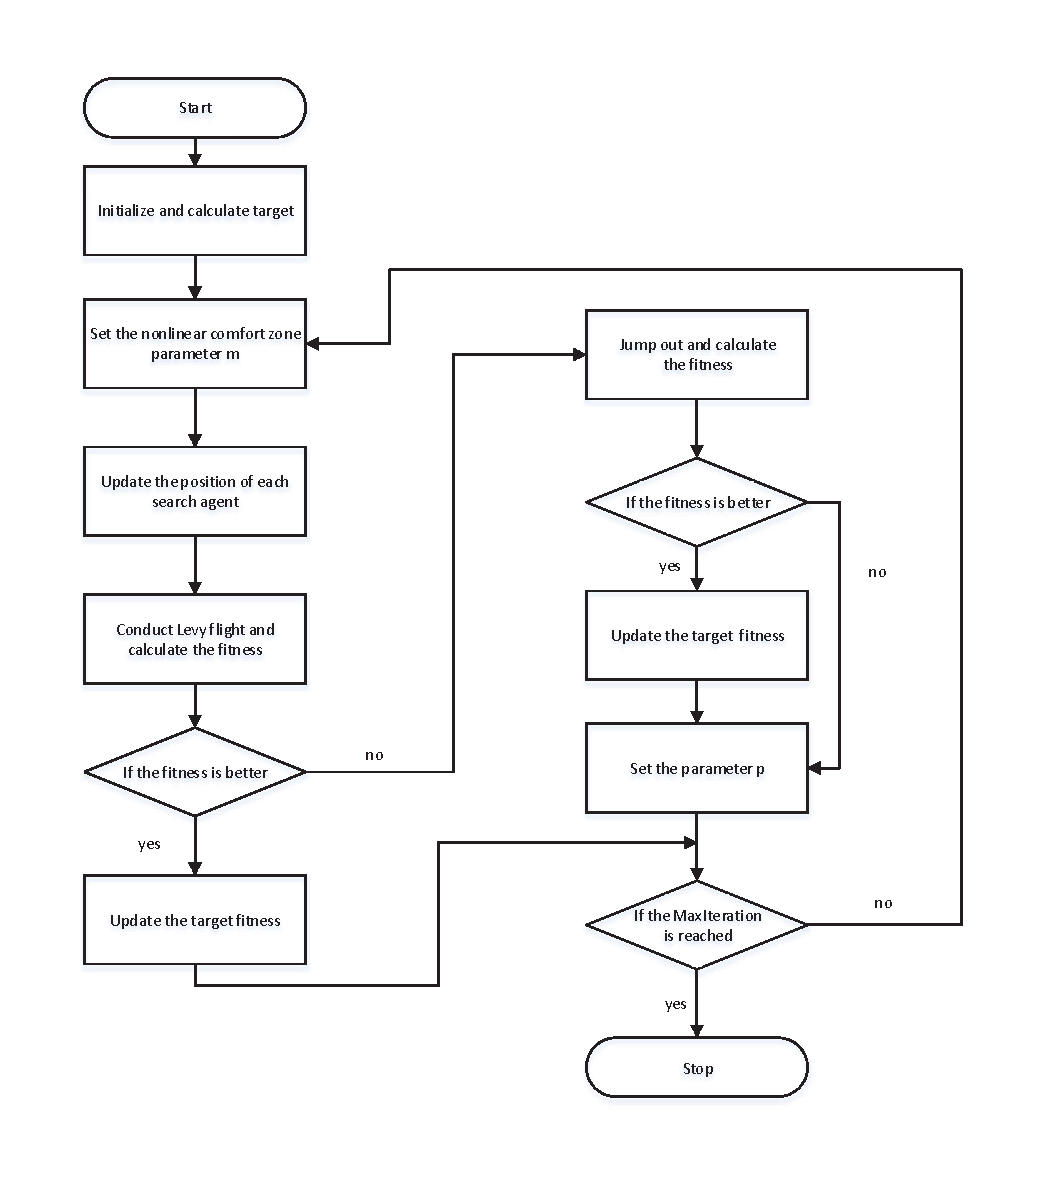
\includegraphics[width=1\linewidth]{procedure_of_IGOA.eps}\hfill\\[0.5cm]
  \caption{The figure framework of the procedure of IGOA}
  \label{fig:procedure_IGOA}
  \end{figure}
\subsection{实验结果}
\subsubsection{实验设置}
为了评估拟议的IGOA的性能,进行了一系列实验。 在这项工作中,IGOA与6个元启发式算法进行了比较,包括原始的Grasshopper优化算法(GOA),基于对立的学习GOA(OBLGOA),最近提出的三种算法,鲸鱼优化算法(WOA),蜻蜓算法(DA) 和Ant Lion Optimizer(ALO),以及经典的启发式算法,粒子群优化算法(PSO)。 将其他6种算法与IGOA相比较的参数设置为论文引用{saremi2017grasshopper,kennedy1995particle,mirjalili2016WOA,mirjalili2016dragonfly,ewees2018改进,mirjalili2015ant}。
% To evaluate the performance of the proposed IGOA, a series of experiments were conducted. In this work, IGOA was compared with 6 meta-heuristic algorithms including the original Grasshopper Optimization Algorithm (GOA), the opposition-based learning GOA (OBLGOA), three recently proposed algorithms, Whale Optimization Algorithm (WOA), Dragonfly Algorithm (DA) and Ant Lion Optimizer (ALO), and a classical heuristic algorithm, Particle Swarm Optimization (PSO). The parameters of the other 6 algorithms compared with IGOA were set as the papers \cite{saremi2017grasshopper,kennedy1995particle,mirjalili2016WOA,mirjalili2016dragonfly,ewees2018improved,mirjalili2015ant} described.
% 这里需要提一下IGOA的参数设置问题

在这一部分中,使用了29个众所周知的基准函数来测试所提出的IGOA的搜索能力。基准测试分为3种类型,可以评估算法的不同功能。在\ref{tab:unimodal_function}中列出的基准\emph{F1-F7}是单峰函数,只有一个最佳位置可以估计开发能力。在\ref{tab:multimodal_function}和\ref{tab:fixedmodal_function}中列出的基准\emph{F8-F23}是具有多个局部最优的多模函数,可以评估探索能力\ cite {saremi2017grasshopper}。在\ref{tab:composite_function}中列出的基准\emph{F24-F29}是复合函数\ cite {liang2005novel},它在框架下组合了一些基本的测试函数,并且更复杂。他们可以评估摆脱局部最优的表现。在\ emph {表1-4}中,\emph{Dim}表示基准函数的维度,\emph{Range}是优化问题的搜索边界,$ f_min $是函数的最佳适应度。
% In this part, 29 well-known benchmark functions were used to test the search ability of the proposed IGOA. The benchmarks are divided into 3 types which can evaluate the different capability of the algorithms. Benchmarks \emph{F1-F7} listed in \emph{Table 1} are unimodal functions with only one optimal location which can estimate the ability of exploitation. Benchmarks \emph{F8-F23} listed in \emph{Table 2} and \emph{Table 3} are multimodal functions with several local optimums which can evaluate the exploration capability \cite{saremi2017grasshopper}.  Benchmarks \emph{F24-F29} listed in \emph{Table 4} are composite functions \cite{liang2005novel} which combine some basic test functions under a framework and are more complicated. They can evaluate the performance of getting out of local optimum. In \emph{Table 1-4}, \emph{Dim} represents the dimension of the benchmark functions, \emph{Range} is the search boundary of the optimization problems, and $f_min$ is the optimal fitness of the functions.

使用Matlab代码进行了与上述29个基准函数相关的一系列实验。 对于\ emph {F1-F23},每个算法使用30个搜索代理进行500次迭代,以进行完整的搜索过程。 对于\ emph {F24-F29},搜索过程包含100次迭代。 每个搜索过程将针对每个算法重复30次以消除意外事件,并且计算一些统计数据,例如平均值(平均值),标准偏差(标准差),最佳适合度30(最佳)和最差适合度30(最差), 比较算法的性能。 此外,进行了Wilcoxon秩和检验,计算了\ emph {p-value}以证明结果的统计显着性。
% A series of experiments relating to the 29 benchmark functions described above were conducted with Matlab code. For \emph{F1-F23}, each algorithm was evolved for 500 iterations with 30 search agents to make a complete search process. For \emph{F24-F29}, a search process contained 100 iterations. Each search process would be repeated 30 times for every algorithm to eliminate contingency and some statistical data, such as average (avg), standard deviation (std), best fitness of 30 (best) and worst fitness of 30 (worst), was calculated to compare the performance of the algorithms. Besides, the Wilcoxon rank-sum test was conducted, and the \emph{p-value} was calculated to demonstrate the statistical significance of the results.

\begin{table}[!htbp]
    \centering
    \caption{fixedmodal functions}
    \label{tab:fixedmodal_function}
    \small
    \renewcommand\arraystretch{2.0} 
    \newcommand{\tabincell}[2]{\begin{tabular}{@{}#1@{}}#2\end{tabular}}
\begin{tabular}{l c c c}
    \hline
    % after \\: \hline or \cline{col1-col2} \cline{col3-col4} ...
    Function & Dim & Range & $f_{min}$ \\
    \hline
    $F_{14}(x)=(\frac{1}{500}+\sum_{j=1}^{25} \frac{1}{j+\sum_{i=1}^2 (x_i-a_{ij})^6})^{-1}$ & 2 & [-65,65]&0 \\
    \hline
    $F_{15}(x)=\sum_{i=1}^{11}[a_i-\frac{x_i(b_i^2+b_ix_2)}{b_i^2+b_ix_3+x_4}]^2$& 4 & [-5,5]&0.00030 \\
    \hline
    $F_{16}(x)=4x_1^2-2.1x_1^4+\frac{1}{3}x_1^6+x_1x_2-4x_2^2+4x_2^4$& 2 & [-5,5] & -1.0316\\
    \hline
    $F_{17}(x)=(x_2-\frac{5.1}{4\pi ^2}x_1^2+\frac{5}{\pi}x_1-6)^2+10(1-\frac{1}{8\pi})\cos x_1+10$& 2 & [-5,5] & 0.3979\\
    \hline
    \tabincell{c}{$F_{18}(x)= [1+(x_1+x_2+1)^2(19-14x_1+3x_1^2-14x_2+6x_1x_2+3x_2^2)]\times$ \\ $[30+2x_1-3x_2)^2\times(18-32x_1+12x_1^2+48x_2-36x_1x_2+27x_2^2)]$ }& 2 & [-2,2] & 3\\
    \hline
    $F_{19}(x)=-\sum_{i=1}^4c_iexp(-\sum_{j=1}^3a_{ij}(x_j-p_{ij})^2)$& 3 & [1,3] & -3.86\\
    \hline
    $F_{20}(x)=-\sum_{i=1}^4c_iexp(-\sum_{j=1}^6a_{ij}(x_j-p_{ij})^2)$& 6 & [0,1] & -3.32\\
    \hline
    $F_{21}(x)=-\sum_{i=1}^5[(X-a_i)(X-a_i)^T+c_i]^{-1}$& 4 & [0,10] & -10.1532\\
    \hline
    $F_{22}(x)=-\sum_{i=1}^7[(X-a_i)(X-a_i)^T+c_i]^{-1}$& 4 & [0,10] & -10.4028\\
    \hline
    $F_{23}(x)=-\sum_{i=1}^10[(X-a_i)(X-a_i)^T+c_i]^{-1}$& 4 & [0,10] & -10.5363\\
    \hline
\end{tabular}
\end{table}

\begin{table}[!htbp]
    \centering
    \caption{Composite functions}
    \label{tab:composite_function}
    \scriptsize
    % \small

\newcommand{\tabincell}[2]{\begin{tabular}{@{}#1@{}}#2\end{tabular}}
    \renewcommand\arraystretch{1.5} 
\begin{tabular}{l c c c}
    \hline
    % after \\: \hline or \cline{col1-col2} \cline{col3-col4} ...
    Function & Dim & Range & $f_{min}$ \\
    \hline
    \tabincell{l}{$F_{24}(CF1)$ \\$f_1,f_2,f_3,...f_{10}=Sphere Function,[\sigma_1,\sigma_2,\sigma_3,...\sigma_{10}=[1,1,1,...1]$\\$[\lambda_1,\lambda_2,\lambda_3,...\lambda_{10}]=[5/100,5/100,5/100,...5/100]$}& 30 & [-5,5]&0 \\
    \hline
    \tabincell{l}{$F_{25}(CF2)$ \\$f_1,f_2,f_3,...f_{10}=Griewank's Function,[\sigma_1,\sigma_2,\sigma_3,...\sigma_{10}=[1,1,1,...1]$\\$[\lambda_1,\lambda_2,\lambda_3,...\lambda_{10}]=[5/100,5/100,5/100,...5/100]$}& 30 & [-5,5]&0 \\
    \hline
    \tabincell{l}{$F_{26}(CF3)$ \\$f_1,f_2,f_3,...f_{10}=Griewank's Function,[\sigma_1,\sigma_2,\sigma_3,...\sigma_{10}=[1,1,1,...1]$\\$[\lambda_1,\lambda_2,\lambda_3,...\lambda_{10}]=[1,1,1,...1]$}& 30 & [-5,5]&0 \\
    \hline
    \tabincell{l}{$F_{27}(CF4)$ \\$f_1,f_2=Ackley's Function,f_3,f_4=Rastrigin's Function,$\\$f_5,f_6=Weierstrass Function,f_7,f_8=Griewank's Function,$\\$f_9,f_{10}=Sphere Function,[\sigma_1,\sigma_2,\sigma_3,...\sigma_{10}=[1,1,1,...1]$\\$[\lambda_1,\lambda_2,\lambda_3,...\lambda_{10}]=[5/32,5/32,5/32,...5/32]$}& 30 & [-5,5]&0 \\
    \hline
    \tabincell{l}{$F_{28}(CF5)$ \\$f_1,f_2=Rastrigin's Function,f_3,f_4=Weierstrass Function,$\\$f_5,f_6=Griewank's Function,f_7,f_8=Ackley's Function,$\\$f_9,f_{10}=Sphere Function,[\sigma_1,\sigma_2,\sigma_3,...\sigma_{10}=[1,1,1,...1]$\\$[\lambda_1,\lambda_2,\lambda_3,...\lambda_{10}]=[1/5,1/5,5/0.5,5/0.5,5/100,5/100,5/32,5/32,5/100,5/100]$}& 30 & [-5,5]&0 \\
    \hline
    \tabincell{l}{$F_{29}(CF6)$ \\$f_1,f_2=Rastrigin's Function,f_3,f_4=Weierstrass Function,$\\$f_5,f_6=Griewank's Function,f_7,f_8=Ackley's Function,$\\$f_9,f_{10}=Sphere Function$\\$[\sigma_1,\sigma_2,\sigma_3,...\sigma_{10}=[0.1,0.2,0.3,0.4,0.5,0.6,0.7,0.8,0.9,1]$\\$[\lambda_1,\lambda_2,\lambda_3,...\lambda_{10}]=[0.1*1/5,0.2*1/5,0.3*5/0.5,0.4*5/0.5,0.5*5/100,$\\$0.6*5/100,0.7*5/32,0.8*5/32,0.9*5/100,1*5/100]$}& 30 & [-5,5]&0 \\
    \hline
  \end{tabular}

\end{table}
\subsubsection{实验结果}
\ emph {F1-F7}是单峰函数,只有一个全局最优,可以测试算法的开发能力。 如果算法具有超强的利用能力,它可以更准确地搜索并找到更接近全局最优的解。\ emph {F1-F7}的结果显示在表\ref{tab:results_unimodal_IGOA}中。
% \emph{F1-F7} are unimodal functions with only one global optimum, which can test the exploitation capability of the algorithms. If an algorithm has a superior ability of exploitation, it can search more accurately and find a solution closer to the global optimum. 


\begin{table}[!htbp]
    \centering
    \caption{Results of unimodal functions}\label{tab:results_unimodal_IGOA}
    \scriptsize
    % \small
    \renewcommand\arraystretch{1.3} 
    \begin{tabular}{*{9}{c}}
    % \toprule
    \hline
    function& type&IGOA&GOA&WOA&DA&ALO&PSO&OBLGOA\\
    \hline
\multirow{4}*{F1}& avg& 3.3538E-15& 0.8386& \textbf{1.0082E-71}& 0.0012& 17.1234&6.6310E-6&2.77E-05\\
    & std&1.9129E-15&0.8473&\textbf{5.3671E-71}&0.0008&17.8648&2.1612E-05&1.57E-05    \\
    & best&8.0120E-16&0.0683&\textbf{5.0175E-87}&0.00010&2.4120&1.5608E-07&7.75E-06    \\
    & worst& 9.1885E-15&4.4591&\textbf{2.9415E-70}&0.0030&78.3488&0.0001&6.68E-05    \\
    \hline
\multirow{4}*{F2}& avg& 2.4358E-08& 10.2444&\textbf{ 1.5782E-51}& 47.0419& 4.9289&0.0953&0.0136\\
    & std&1.0173E-08&22.2516&\textbf{4.8668E-51}&43.4815&3.7734&3.0196E-01&0.0377    \\
    & best&9.0029E-09&0.0290&\textbf{2.5368E-57}&3.8197&1.4484&0.0003&0.0011    \\
    & worst&5.7194E-08&79.1046&\textbf{2.1838E-50}&120.4026&21.3472&1.6419&0.1505    \\
    \hline
\multirow{4}*{F3}& avg&0.0121& 1789.3452&43942.9825&4632.0793&1154.2060&227.7776 &\textbf{0.0061}\\
    & std&0.0211&	1030.4488&1.6119E+04&2008.3302&1332.5907&81.0377&\textbf{0.0021}    \\
    & best&\textbf{8.6626E-12}&450.4535&17269.6957&1883.2010&249.1874&127.3043&0.0020    \\
    & worst&0.0983&4603.9086&85296.2126&10156.9819&5729.0798&425.9704&\textbf{0.0103}    \\
    \hline
\multirow{4}*{F4}& avg&0.0257&9.7756&56.3543&16.9378&31.4847&3.2311&\textbf{0.0165}\\
    & std&0.0182&3.5013&25.3903&4.3129&8.2314&1.1774&\textbf{0.0081}    \\
    & best&\textbf{9.7116E-7}&3.0335&3.2199&6.5808&17.7108&1.4918&0.0010    \\
    & worst&0.0694&19.5647&89.1869&57.2014&48.8229&5.5785&\textbf{0.0297}    \\
    \hline
\multirow{4}*{F5}& avg&\textbf{26.4488}&965.6578&28.1591&348.5174&1615.4578&61.9257&28.3790\\
    & std&\textbf{0.3046}&1572.3600&0.4797&553.5976&2814.6516&64.9991&0.3087    \\
    & best&25.8503&25.6988&27.2726&28.4537&143.9488&\textbf{1.7275}&27.6749    \\
    & worst&\textbf{27.0365}&7522.9967&28.7708&2223.6927&14636.9499&268.0065&28.7678    \\
    \hline
\multirow{4}*{F6}& avg&\textbf{1.4451E-6}& 0.8997&0.3866&0.0023&20.5677&2.2973E-05&1.2542\\
    & std&\textbf{4.8437E-7}&2.0343&0.2498&0.0055&29.2793&5.0099E-05&0.4237    \\
    & best&\textbf{5.2803E-7}&0.0203&0.0856&0.0001&3.0268&1.5390E-07&0.6616    \\
    & worst& \textbf{2.5210E-6}&11.0963&1.0626&0.0306&148.1366&0.0002&2.1687    \\
    \hline
\multirow{4}*{F7}& avg& \textbf{0.0010}&0.0234&0.0032&0.2504&0.1588&0.0274&0.0014\\
    & std&\textbf{0.0014}&0.0106&0.0032&0.0768&0.0934&0.0113&0.0007    \\
    & best&\textbf{1.0746E-5}&0.0090&5.1138E-5&0.1003&0.0467&0.0115&0.0006    \\
    & worst&0.0072&0.0602&0.0118&0.4105&0.3750&0.0538&\textbf{0.0033}    \\
    \hline
    % \bottomrule
    \end{tabular}
    \end{table}

从表\ref{tab:results_unimodal_IGOA}可以看出,IGOA可以在\ emph {F5-F7}中获得最佳平均结果,并且在\ emph {F1-F4}中,IGOA的表现仅比WOA差。 至于std和最差值,IGOA也可以比\ emph {F3-F7}中的其他算法表现更好,这表明所提出的算法可以降低获得可怕解的可能性并提高算法的稳定性。 与GOA和OBLGOA相比,提出的IGOA可以显着提高原算法的开发能力。
% The results on \emph{F1-F7} are shown in \emph{Table 5}. It could be seen that IGOA could get the best average results in \emph{F5-F7}, and in \emph{F1-F4} IGOA behaved only worse than WOA. As for std and worst value, IGOA could also perform better than the other algorithms in \emph{F3-F7}, which indicates that the proposed algorithm can reduce the probability of getting terrible solutions and promote the stability of the algorithm. Compared with GOA and OBLGOA, the proposed IGOA can significantly improve the exploitation capability of the original algorithm.  

\emph{F8-F23}是具有多个局部最优的多模函数,可以测试算法的探索能力。 如果算法在探索中不能很好地进行,那么在处理多模态函数时,搜索很可能会陷入局部最优,即使最佳的利用能力也无济于事。 错误的方向可能会导致错误的结果。\ emph {F8-F23}的结果显示在\ emph {表6}和\ emph {表7}中。
% \emph{F8-F23} are multimodal functions with several local optimums, which can test the exploration capability of the algorithms. If an algorithm cannot do well in exploration, the search will most likely fall into local optimum when dealing with the multimodal functions and even the best ability of exploitation cannot help. A wrong direction can probably lead to a wrong result. 


\begin{table}[!htbp]
    \centering
    \caption{Results of multimodal functions-1}\label{tab:results_multimodal_IGOA}
    \scriptsize
    % \small
    \renewcommand\arraystretch{1.3} 
    \begin{tabular}{*{9}{c}}
        % \toprule
    \hline
    function& type&IGOA&GOA&WOA&DA&ALO&PSO&OBLGOA\\
    \hline
    \multirow{4}*{F8}&avg & -7594.1662 & -7728.4324 & \textbf{-9969.6875} & -6189.11 & -7320.0609 & -6688.3058&-7901.9216\\
        & std & 767.0277 & \textbf{593.4825} & 1919.0327 & 1833.8338 & 886.1388 & 684.8647&591.8701    \\
        & best & -9009.3177 & -8903.0523 & -12564.8051 & \textbf{-12568.5831} & -9628.8472 & -7869.7845&-9598.7278    \\
        & worst& -5993.9317 & -6468.5651 & -5709.2023 & -5417.6748 & -6101.1009 & -5224.2865&\textbf{-6823.4703}    \\
        \hline
    \multirow{4}*{F9}& avg& \textbf{0.0000} & 9.4853 & 0.4119 & 8.8883 & 7.4670 & 4.5109&1.7919\\
        & std& \textbf{0.0000} & 5.4604 & 1.6505 & 4.5100 & 4.1855 & 2.8231 &2.1937    \\
        & best& \textbf{0.0000} & 1.9899 & 0.0000 & 0.9950 & 0.9959 & 0.9950 &4.42E-09    \\
        & worst& \textbf{0.0000} & 27.8586 & 8.1471 & 16.9143 & 16.9159 & 10.9445&6.9648    \\
        \hline
    \multirow{4}*{F10}& avg& 1.30e-08 & 3.0892 & \textbf{4.56e-15} & 5.0040 & 9.9207 & 1.3594&0.0010\\
        & std& 3.13e-09 & 0.8305 & \textbf{2.18e-15} & 3.1845 & 3.9783 & 0.8583&0.0002    \\
        & best& 8.58e-09 & 1.5021 & \textbf{8.88e-16} & 1.1582 & 3.3950 & 0.0002&0.0005    \\
        & worst& 1.97e-08 & 4.5855 & \textbf{7.99e-15} & 12.3302 & 16.3216 & 2.8857&0.0015    \\
        \hline
    \multirow{4}*{F11}& avg& \textbf{5.50e-15} & 0.6966 & 0.0069 & 0.0610 & 1.1803 & 0.0258&0.0002\\
        & std& \textbf{5.71e-15} & 0.1924 & 0.0379 & 0.0268 & 0.1822 & 0.0354&8.83E-05    \\
        & best& \textbf{6.66e-16} & 0.3226 & 0.0000 & 0.0068 & 1.041 & 9.58e-07&7.36E-05    \\
        & worst& \textbf{2.52e-14} & 1.0411 & 0.2076 & 0.1151 & 1.9360 & 0.1590&0.0004    \\
        \hline
    \multirow{4}*{F12}& avg& \textbf{8.93e-08} & 5.6658 & 0.0242 & 14.9630 & 25.6688 & 0.5808&0.0347\\
        & std& \textbf{3.28e-08} & 2.3767 & 0.0162 & 7.2414 & 14.1457 & 0.8898&0.0211    \\
        & best& \textbf{4.62e-08} & 1.8994 & 0.004 & 6.9778 & 6.3337 & 1.89e-07&0.0051    \\
        & worst& \textbf{1.85e-07} & 9.7664 & 0.0832 & 35.5319 & 55.4036 & 3.4350&0.1028    \\
        \hline
    \multirow{4}*{F13}& avg& \textbf{0.0138} & 8.7624 & 0.6039 & 24.9054 & 261.6986 & 0.2117&0.4087\\
        & std& \textbf{0.0298} & 9.0372 & 0.2536 & 15.4205 & 1186.8265 & 0.5112&0.2177    \\
        & best& \textbf{4.85e-07} & 0.3005 & 0.1459 & 0.3854 & 1.3788 & 9.86e-07&0.1211    \\
        & worst& \textbf{0.0989} & 35.2838 & 1.2995 & 56.9980 & 6534.7729 & 2.0239&1.1019    \\
        \hline
        % \bottomrule
    \end{tabular}
\end{table}
\begin{table}[!htbp]
    \centering
    \caption{Results of fixedmodal functions}\label{tab:results_fixedmodal_IGOA}
    \scriptsize
    % \small
    \renewcommand\arraystretch{1.3} 
    \begin{tabular}{*{9}{c}}
        % \toprule
    \hline
    function& type&IGOA&GOA&WOA&DA&ALO&PSO&OBLGOA\\
    \hline
    \multirow{4}*{F14}&avg & 3.5566& \textbf{0.9980} & 2.7622 & 2.2142 & 1.7242 & 4.5076&3.0103\\
        & std & 2.9933 & \textbf{6.4341e-16} & 3.3587 & 2.1646 & 1.2701 & 3.0100&1.5672    \\
        & best & \textbf{0.9980} & 0.9980 & 0.9980 & 0.9980 & 0.9980 & 0.9980&0.9980    \\
        & worst & 10.7632    & \textbf{0.9980} & 10.7632 & 10.7632 & 5.9288 & 12.6705&5.9288    \\
        \hline
    \multirow{4}*{F15}& avg& \textbf{0.0003}& 0.0071 & 0.0007 & 0.0032 & 0.0029 & 0.0038&0.0063\\
        & std& \textbf{3.24E-05}    & 0.0089 & 0.0005 & 0.0062 & 0.0059 & 0.0076&0.0087    \\
        & best& \textbf{0.0003} & 0.0007 & 0.0003 & 0.0006 & 0.0003 & 0.0003&0.0003    \\
        & worst& \textbf{0.0004}    & 0.0204 & 0.0022 & 0.0206 & 0.0204 & 0.0204&0.0210    \\
        \hline
    \multirow{4}*{F16}& avg& \textbf{-1.0316} & -1.0316 & -1.03162 & -1.0316 & -1.0316 & -1.0316&-1.0316\\
        & std& \textbf{4.44E-16}    & 8.1630e-13 & 1.6137e-09 & 1.0917e-13 & 5.1620e-07 & 6.5195e-16&4.63E-06    \\
        & best & \textbf{-1.0316} & -1.0316 & -1.0316 & -1.0316 & -1.0316 & -1.0316&-1.0316    \\
        & worst& \textbf{-1.0316} & -1.0316 & -1.0316 & -1.0316 & -1.0316 & -1.0316&-1.0316    \\
        \hline
    \multirow{4}*{F17}& avg& \textbf{0.3979} & 0.3979 & 0.3979 & 0.3979 & 0.3979 & 0.3979&0.3979\\
        & std& \textbf{0}    & 7.3750e-13 & 8.4140e-06 & 2.1005e-14 & 1.0879e-06 & 0.0000 &1.82E-06    \\
        & best& \textbf{0.3979} & 0.3979 & 0.3979 & 0.3979 & 0.3979 & 0.3979&0.3979    \\
        & worst& \textbf{0.3979} & 0.3979 & 0.3979 & 0.3979 & 0.3979 & 0.3979&0.3979 \\
        \hline
    \multirow{4}*{F18}&avg & \textbf{3.0000} & 8.4000 & 3.0000 & 3.0000 & 3.0000 & 3.0000&3.0000\\
        & std& 4.11E-08    & 20.5503 & 7.0794e-05 & 6.2232e-13 & 7.7233e-06 & \textbf{6.0036e-16}&3.07E-10    \\
        & best& \textbf{3.0000} & 3.0000 & 3.0000 & 3.0000 & 3.0000 & 3.0000&3.0000\\
        & worst& \textbf{3.0000} & 84.0000 & 3.0003 & 3.0000 & 3.0000 & 3.0000&3.0000 \\
        \hline
    \multirow{4}*{F19}& avg& \textbf{-3.8628}& -3.7288 & -3.8582 & -3.8628 & -3.8628 & -3.8628&-3.8628\\
        & std& 1.67E-10    & 0.3062 & 0.0054 & 2.4040e-13 & 2.2464e-05 & \textbf{2.6402e-15}&2.95E-05    \\
        & best& \textbf{-3.8628} & -3.8628 & -3.8628 & -3.8628 & -3.8628 & -3.8628&-3.8628  \\
        & worst& \textbf{-3.8628}    & -2.7847 & -3.8408 & -3.8628 & -3.8627 & -3.8628&-3.8627 \\
        \hline
    \multirow{4}*{F20}& avg& -3.2863& \textbf{-3.2943} & -3.2364 & -3.2621 & -3.2819 & -3.2783&-3.2295\\
        & std& 0.0554    & \textbf{0.0511} & 0.1007 & 0.0610 & 0.0577 & 0.0584&0.1062    \\
        & best& \textbf{-3.3220} & -3.3220 & -3.3213 & -3.3220 & -3.3220 & -3.3220&-3.3220    \\
        & worst& \textbf{-3.2031} & -3.2031 & -3.0184 & -3.1981 & -3.1974 & -3.1996&-3.0334    \\
        \hline
        \hline
    \end{tabular}
\end{table}
\begin{table}[!htbp]
    \ContinuedFloat% continue splited float
    \centering
    \caption{续表:Results of fixedmodal functions}\label{tab:results_fixedmodal_IGOA}
    \small
    \renewcommand\arraystretch{1.3} 
    \begin{tabular}{*{9}{c}}
    \multirow{4}*{F21}& avg& \textbf{-8.2870}& -6.0675 & -8.5287 & -5.8753 & -6.6400 & -5.9796&-7.2158\\
        & std& \textbf{2.4947}    & 3.6827 & 2.7585 & 3.0237 & 3.2604 & 3.3646&3.3058    \\
        & best& \textbf{-10.1532} & -10.1532 & -10.1498 & -10.1532 & -10.1532 & -10.1532&-10.1532    \\
        & worst& \textbf{-5.0552} & -2.6305 & -2.6292 & -2.6305 & -2.6305 & -2.6305&-2.6303    \\
        \hline
    \multirow{4}*{F22}& avg& \textbf{-9.3413}& -7.1190 & -7.2448 & -7.1785 & -5.1249 & -5.5091&-8.0724\\
        & std& \textbf{2.1597}    & 3.6556 & 3.0850 & 3.3668 & 2.5737 & 3.1769&3.1972    \\
        & best& \textbf{-10.4029} & -10.4029 & -10.4020 & -10.4029 & -10.4029 & -10.4029&-10.4029    \\
        & worst& \textbf{-5.0877}    & -1.8376 & -1.8352 & -1.8376 & -2.7517 & -1.8376&-2.7658    \\
        \hline
    \multirow{4}*{F23}& avg& -7.9281& -4.9279 & -6.5554 & -6.6569 & -5.4597 & -4.7287&\textbf{-8.0791}\\
        & std& \textbf{2.8536}    & 3.2796 & 3.3755 & 3.7558 & 3.0183 & 3.2997&3.5845    \\
        & best& \textbf{-10.5364} & -10.5364 & -10.5348 & -10.5364 & -10.5364 & -10.5364&-10.5364    \\
        & worst& \textbf{-3.8354} & -2.4217 & -1.6721 & -2.4217 & -2.4217 & -2.4273&-2.4217    \\
        \hline
        % \bottomrule
    \end{tabular}
\end{table}
从表\ref{tab:results_multimodal_IGOA}和表\ref{tab:results_fixedmodal_IGOA}中可以发现,提议的IGOA可以在16个基准测试中的11个中获得最佳平均适应度,并且在\ emph {F10},\ emph {F20}和\ emph {23} IGOA可以获得第二好的结果。 关于标准偏差的结果表明,IGOA的稳定性可能不如平均适应度所表现的那么好,但在大多数测试中它仍然是所有7种算法中最好的。 关于最佳适应度和最差适应度的结果可以表明,所提出的IGOA具有在几乎所有基准测试中找到最佳解决方案的最可靠能力,并且获得找到最差解决方案的最小概率。 与原始的GOA和OBLGOA相比,提出的IGOA可以自然地提高算法的探索性能。
% The results on \emph{F8-F23} are presented in \emph{Table 6} and \emph{Table 7}. It can be found that the proposed IGOA can get the best average fitness in 11 of 16 benchmark tests and in \emph{F10}, \emph{F20} and \emph{23} IGOA can get the second best result. The results about standard deviation show that the stability of IGOA might not be as excellent as it shows in average fitness, but it still is the best of all the 7 algorithms in most of the tests. The results on best fitness and worst fitness can show that the proposed IGOA has the most reliable ability to find the best solution in almost all the benchmark tests and get the minimum probability to find the worst solution. In comparison with the original GOA and OBLGOA, the proposed IGOA can naturally enhance the performance of exploration of the algorithm a lot.


\emph{F24-F29}是复合测试函数,它结合了特定框架下的一些基本基准函数来构建新的可控测试函数。 复合基准函数比多模式测试函数更复杂,更具挑战性,并且在评估算法的搜索能力时更有说服力。复合测试函数的结果如表\ref{tab:results_composite_IGOA}所示:
% \emph{F24-F29} are the composite test functions, which combine some basic benchmark functions under a particular framework to construct new controllable test functions. The composite benchmark functions are more complicated and more challenging than multimodal test functions, and they are more convincing when evaluating the search capability of an algorithm. 


\begin{table}[!htbp]
    \centering
    \caption{Results of composite functions}\label{tab:results_composite_IGOA}
    \scriptsize
    % \small
    \renewcommand\arraystretch{1.3} 
\begin{tabular}{*{9}{c}}
    % \toprule
    \hline
    function& type&IGOA&GOA&WOA&DA&ALO&PSO&OBLGOA\\
    \hline
\multirow{4}*{F24}& avg& \textbf{94.0428} & 135.9242 & 341.2250 & 1098.8600 & 189.5840 & 326.5899&189.6304\\
    & std& 130.6690 & 127.0964 & 164.2449 & \textbf{99.4449} & 117.6155 & 149.6609&83.2598    \\
    & best& \textbf{3.3965} & 29.6057 & 163.2687 & 796.3368 & 72.0563 & 118.9426&92.1210    \\
    & worst& 504.8393 & 514.7878 & 844.9761 & 1261.1685 & 554.4573 & 717.0723&\textbf{411.3461}    \\
    \hline
\multirow{4}*{F25}& avg& 324.3197 & \textbf{284.6066} & 521.9304 & 1211.2487 & 413.5431 & 393.6293&472.0768\\
    & std& 151.6351 & 163.1829 & 130.9867 & \textbf{94.2232} & 156.9269 & 126.4408&143.6411    \\
    & best& \textbf{21.2736} & 28.9418 & 244.2571 & 1006.3367 & 72.6341 & 161.9665&66.0628    \\
    & worst& \textbf{497.3555} & 510.3606 & 673.6729 & 1354.7747 & 662.1609 & 610.8645&606.4133    \\
    \hline
\multirow{4}*{F26}& avg& \textbf{525.7384} & 624.5092 & 1052.0733 & 1547.6195 & 884.9306 & 608.4939&875.4033\\
    & std& 128.5247 & 176.1401 & 155.6153 & 155.8894 & 157.8576 & \textbf{103.4249}&151.2467    \\
    & best& 317.4166 & \textbf{200.8044} & 849.0492 & 1064.4776 & 644.6867 & 326.5611&627.7263    \\
    & worst & 900.011 & 1196.9114 & 1351.5909 & 1710.9641 & 1222.5593 & \textbf{828.4274}&1217.9587    \\
    \hline
\multirow{4}*{F27}& avg& 894.6861 & 945.6744 & 902.6182 & 1421.5043 & 929.5948 & \textbf{757.5836}&895.7587\\
    & std& 29.1104 & 101.1013 & \textbf{15.0373} & 46.9584 & 128.2259 & 114.6504&34.7088    \\
    & best& 740.5569 & 638.304 & 896.3862 & 1319.5644 & 650.1341 & \textbf{538.8135}&719.3590    \\
    & worst& \textbf{900.0053} & 1030.5605 & 982.1588 & 1519.1409 & 1066.455 & 1012.7758 &953.3374    \\
    \hline
\multirow{4}*{F28}& avg & 304.9727 & \textbf{142.0615} & 456.9052 & 1354.378 & 194.2336 & 303.9595&497.1264\\
    & std& 367.9136 & \textbf{102.2128} & 255.4945 & 127.0279 & 182.4486 & 143.7137&351.6947    \\
    & best& \textbf{46.3796} & 54.2782 & 179.8317 & 992.2916 & 87.2393 & 113.7433&110.5681    \\
    & worst& 900.0040 & \textbf{435.4893} & 900.0000 & 1505.6248 & 1025.2583 & 675.3012&900.0049    \\
    \hline
\multirow{4}*{F29}& avg& 900.0003 & 907.4664 & \textbf{900.0000} & 1371.4241 & 925.7089 & 931.1013&900.0004 \\
    & std& 0.0001 & 5.1380 & \textbf{0.0000} & 56.4060 & 7.5901 & 19.0467&0.0002\\
    & best& \textbf{900.0000} & 901.0860 & 900.0000 & 1254.6648 & 913.0986 & 910.3009&900.0001 \\
    & worst& 900.0006 & 920.7888 & \textbf{900.0000} & 1000.7252 & 1000.7252 & 1000.7252&900.0009\\
    \hline
    % \bottomrule
\end{tabular}
\end{table}
根据表\ref{tab:results_composite_IGOA}中列出的\emph{F24-F29}的结果,可以看出,与其他算法相比,所提出的IGOA可以非常有竞争力。 在\emph{F24}和\emph{F26}中,IGOA可以获得最佳的适应度,在\emph{F25},\emph{F27}和\emph{F29} IGOA可以获得第二好的结果。 在所有基准测试的标准差方面,IGOA无法表现最佳或最差。 IGOA在最佳值和最差值上分别在4次测试和3次测试中表现最佳。 尽管IGOA通常可以在标准偏差方面发挥作用,但它在寻找更好的解决方案和控制风险方面可以胜过其他算法。 与原来的GOA和OBLGOA相比,IGOA的表现要好得多。 根据复合功能测试的结果,可以证明IGOA具有处理这种复杂和具有挑战性的问题的能力。

% According to the results on \emph{F24-F29} listed in \emph{Table 8}, it can be seen that the proposed IGOA can be very competitive compared with the other algorithms. In \emph{F24} and \emph{F26} IGOA can get the best fitness and in \emph{F25}, \emph{F27} and \emph{F29} IGOA can get the second-best results. IGOA cannot perform best nor worst in the aspect of the standard deviation on all the benchmark tests. IGOA can perform best in 4 tests and 3 tests respectively on best value and worst value. Although IGOA can perform generally in terms of standard deviation, it can outperform other algorithms in the potency of finding a better solution and controlling risk. Compared with the original GOA and the OBLGOA, IGOA performs far better. According to the results on composite function tests, it can be demonstrated that IGOA has the ability to handle such complex and challenging problems.
\subsubsection{wilcoxon秩和检验}

基于30个独立操作的平均值和标准偏差的比较没有比较每个操作之间的差异。 实验结果仍有可能包含某些意外情况。 为了消除这种偶然性并证明实验结果的重要性,在这项工作中引入了Wilcoxon秩和检验。 Wilcoxon秩和检验是零假设的非参数检验,它用于确定两个独立的数据集是否来自相同的分布式群体。 在这项工作中,计算了关于IGOA与\emph{F1-F29}上的每个其他算法之间的统计数据的\emph{p-values}。 当\emph{p-value}小于0.05时,可以认为两个样本之间的差异是显着的。IGOA的威尔科克森秩和检验结果如表\ref{tab:results_wilcoxon_rank_sum_test_IGOA}所示。
% The comparison based on average value and standard deviation for 30 independent operations did not compare the difference between each operation. It was still possible that the results of the experiment contained certain contingency. To dispel this contingency and demonstrate the significance of the results of the experiment, the Wilcoxon rank-sum test was introduced in this work. Wilcoxon rank-sum test is a nonparametric test of the null hypothesis, and it is used to determine whether two independent datasets were from the same distributed population. In this work, \emph{p-values} about the statistical data between IGOA and each of the other algorithms on \emph{F1-F29} were calculated. When \emph{p-value} is less than 0.05, it can be considered that the difference between the two samples is significant.


\begin{table}%[!htbp]
    \centering
    \caption{Results of Wilcoxon rank-sum test}\label{tab:results_wilcoxon_rank_sum_test_IGOA}
    \renewcommand\arraystretch{1.3} 

	% \tiny

    \begin{tabular}{*{7}{c}}
    % \toprule
    \hline
    function&GOA&WOA&DA&ALO&PSO&OBLGOA\\
    \hline
 
    {F1}& 3.02E-11&3.02E-11&3.02E-11&3.02E-11&9.53E-07&2.03E-07\\\hline
    {F2}& 3.02E-11&3.02E-11&3.02E-11&3.02E-11&7.12E-09&2.37E-10\\\hline
    {F3}& 3.02E-11&3.02E-11&3.02E-11&3.02E-11&3.02E-11&5.57E-10\\\hline
    {F4}& 3.02E-11&3.02E-11&3.02E-11&3.02E-11&3.02E-11&1.21E-10\\\hline
    {F5}& 1.86E-09&1.60E-07&3.02E-11&3.02E-11&0.5201&5.07E-10\\\hline
    {F6}& 3.02E-11&3.02E-11&3.02E-11&0.0099&3.02E-11&3.02E-11\\\hline
    {F7}& 3.16E-10&0.7618&3.02E-11&3.02E-11&8.15E-11&0.0594\\\hline
    {F8}& 0.0030&3.82E-09&0.7958&2.59E-06&0.0133&0.0002\\\hline
    {F9}& 3.02E-11&1.24E-09&3.02E-11&3.02E-11&2.86E-11&4.98E-11\\\hline
    {F10}& 3.02E-11&3.02E-11&3.02E-11&3.02E-11&1.43E-08&3.83E-05\\\hline
    {F11}& 3.02E-11&4.56E-11&3.02E-11&3.02E-11&1.34E-05&3.02E-11\\\hline
    {F12}& 3.02E-11&3.02E-11&3.02E-11&3.02E-11&0.0002&3.02E-11\\\hline
    {F13}& 3.02E-11&3.02E-11&3.02E-11&3.02E-11&0.9117&3.02E-11\\\hline
    {F14}& 1.67E-05&0.1578&0.0265&0.0082&0.7842&0.6951\\\hline
    {F15}& 1.33E-10&1.07E-09&2.87E-10&2.87E-10&0.3328&2.15E-10\\\hline
    {F16}& 0.0064&6.72E-10&3.02E-11&1.81E-05&4.08E-12&3.02E-11\\\hline
    {F17}& 3.20E-06&3.01E-11&3.01E-11&6.78E-06&4.56E-12&3.01E-11\\\hline
    {F18}& 1.73E-07&3.02E-11&3.02E-11&0.01911&1.55E-11&5.09E-08\\\hline
    {F19}& 0.5997&0.002266&2.13E-05&3.33E-11&5.14E-12&0.0003\\\hline
    {F20}& 0.5395&0.0003&0.00250&0.7958&0.0003&0.0001\\\hline
    \end{tabular}
\end{table}
\begin{table}[!htbp]
    \ContinuedFloat% continue splited float
    \centering
    \caption{续表:Results of Wilcoxon rank-sum test}\label{tab:results_wilcoxon_rank_sum_test_IGOA}
    % \scriptsize
    % \small
    \renewcommand\arraystretch{1.3} 
    \begin{tabular}{*{7}{c}}
    {F21}& 0.0002&1.25E-05&6.74E-06&0.0850&0.2822&5.46E-06\\\hline
    {F22}& 0.0005&5.27E-05&3.83E-06&0.5493&0.0627&0.0013\\\hline
    {F23}& 6.05E-07&3.83E-06&1.73E-06&0.1858&0.0009&5.27E-05\\\hline
    {F24}& 0.0016&6.01E-08&0.0001&3.02E-11&3.81E-07&0.0001\\\hline
    {F25}& 0.7618&1.09E-05&0.0138&3.02E-11&0.1907&1.02E-05\\\hline
    {F26}& 0.0046&5.49E-11&5.57E-10&3.02E-11&0.0038&4.20E-10\\\hline
    {F27}& 7.74E-06&7.34E-09&0.0064&3.02E-11&3.08E-08&2.68E-06\\\hline
    {F28}& 0.3711&0.0042&0.0083&3.02E-11&0.0073&0.0001\\\hline
    {F29}& 3.02E-11&2.14E-11&3.02E-11&3.02E-11&3.02E-11&0.0024\\\hline
    
    % \bottomrule
\end{tabular}
\end{table}

从\ref{tab:results_wilcoxon_rank_sum_test_IGOA}中可以看出,在大多数基准测试中,IGOA与另一个比较算法之间的\emph {p-values}小于0.05。 在某些测试函数中,某些\emph{p-values}超过0.05,这些函数通过不同的算法获得相同的最优解,例如\emph{F14,F19,F20,F21,F22}和\emph{F23}。 通过分析复合函数的结果,在\emph{F25}和\emph{F28}中,\emph{p-values}在IGOA和GOA之间超过0.05,其中GOA获得最佳适应度而IGOA没有。综合考虑,仍然可以证明提议的IGOA可以显着提高GOA的性能。
% From \emph{Table 9} it can be seen that the \emph{p-values} between IGOA and another compared algorithm in most of the benchmark tests are less than 0.05. Some \emph{p-values} are more than 0.05 in some of the test functions which have a higher probability of achieving the same optimal solution by different algorithms, such as \emph{F14,F19,F20,F21,F22,} and \emph{F23}. By analyzing the results of the composite functions, \emph{p-values} are more than 0.05 between IGOA and GOA in \emph{F25} and \emph{F28} where GOA gets the best fitness and IGOA does not. Considering comprehensively, it can still be demonstrated that the proposed IGOA can significantly promote the performance of GOA.
\subsubsection{收敛图}

本部分讨论了算法的收敛速度。用于比较部分基准函数的IGOA和所有其他6种算法的收敛曲线显示在\ emph {图2}中。
\pagestyle{empty}
\graphicspath{{Img/}}
\begin{figure}[htbp]
    \centering
    % \includegraphics[width=.25\linewidth]{function_F2.eps}\hfill
    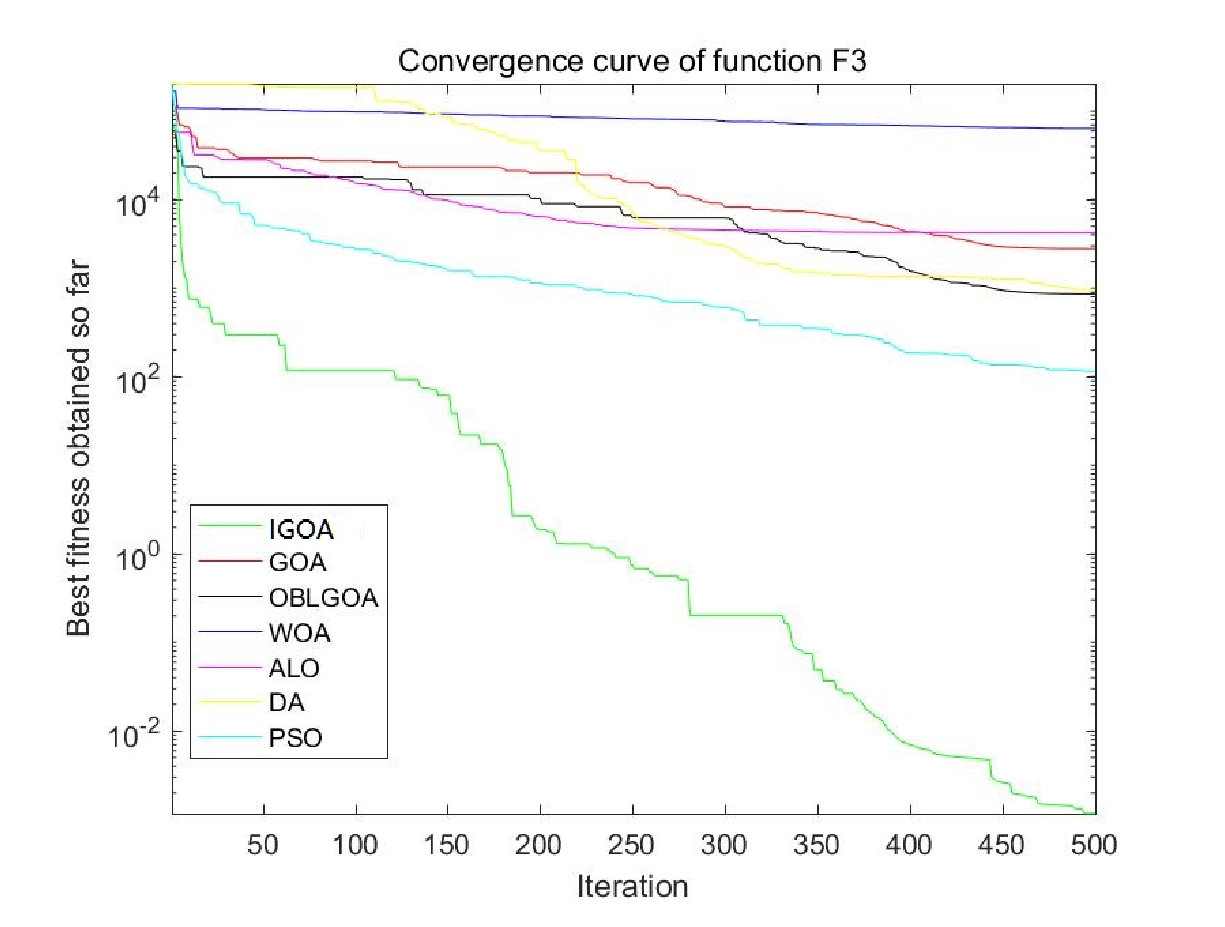
\includegraphics[width=.33\linewidth]{function_F3.eps}\hfill
    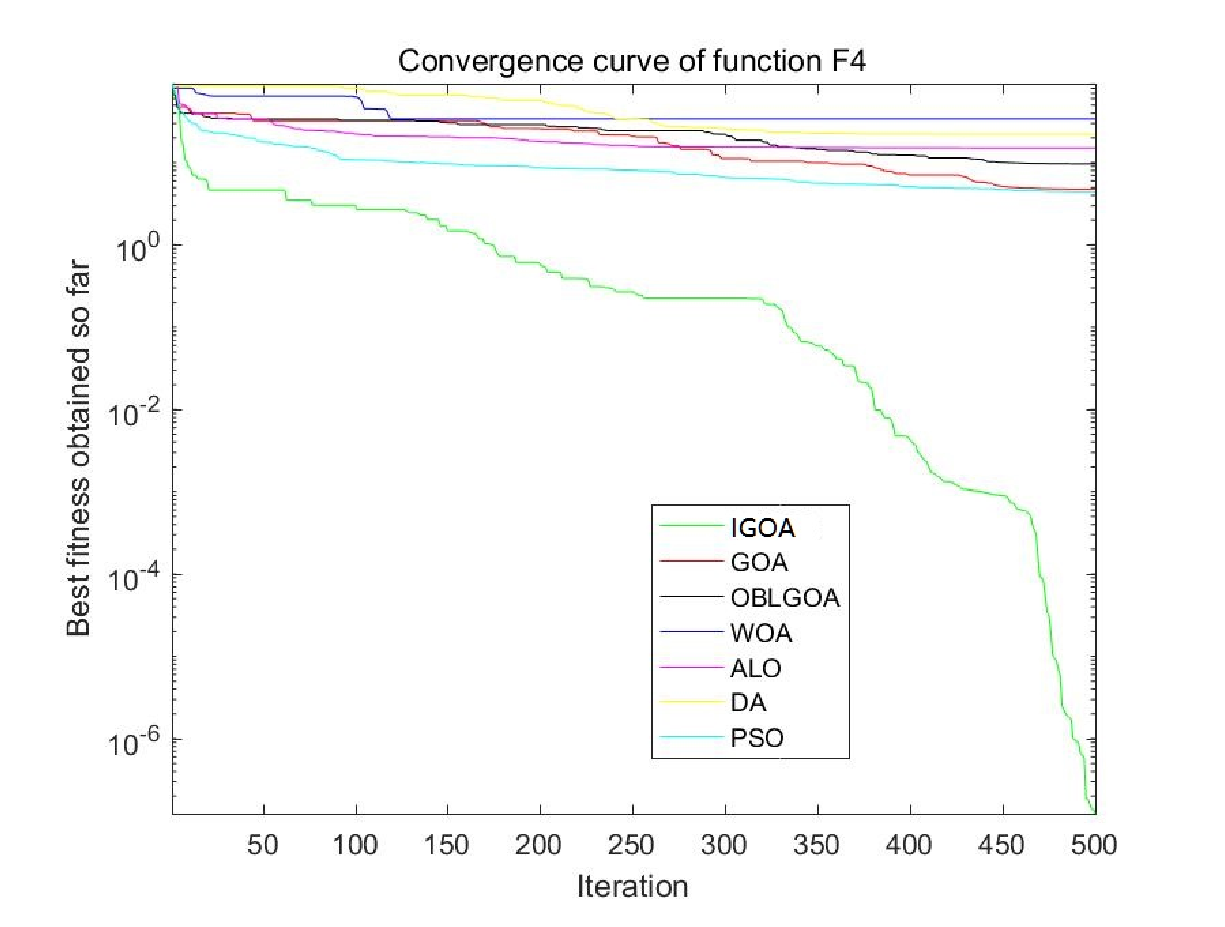
\includegraphics[width=.33\linewidth]{function_F4.eps}\hfill
    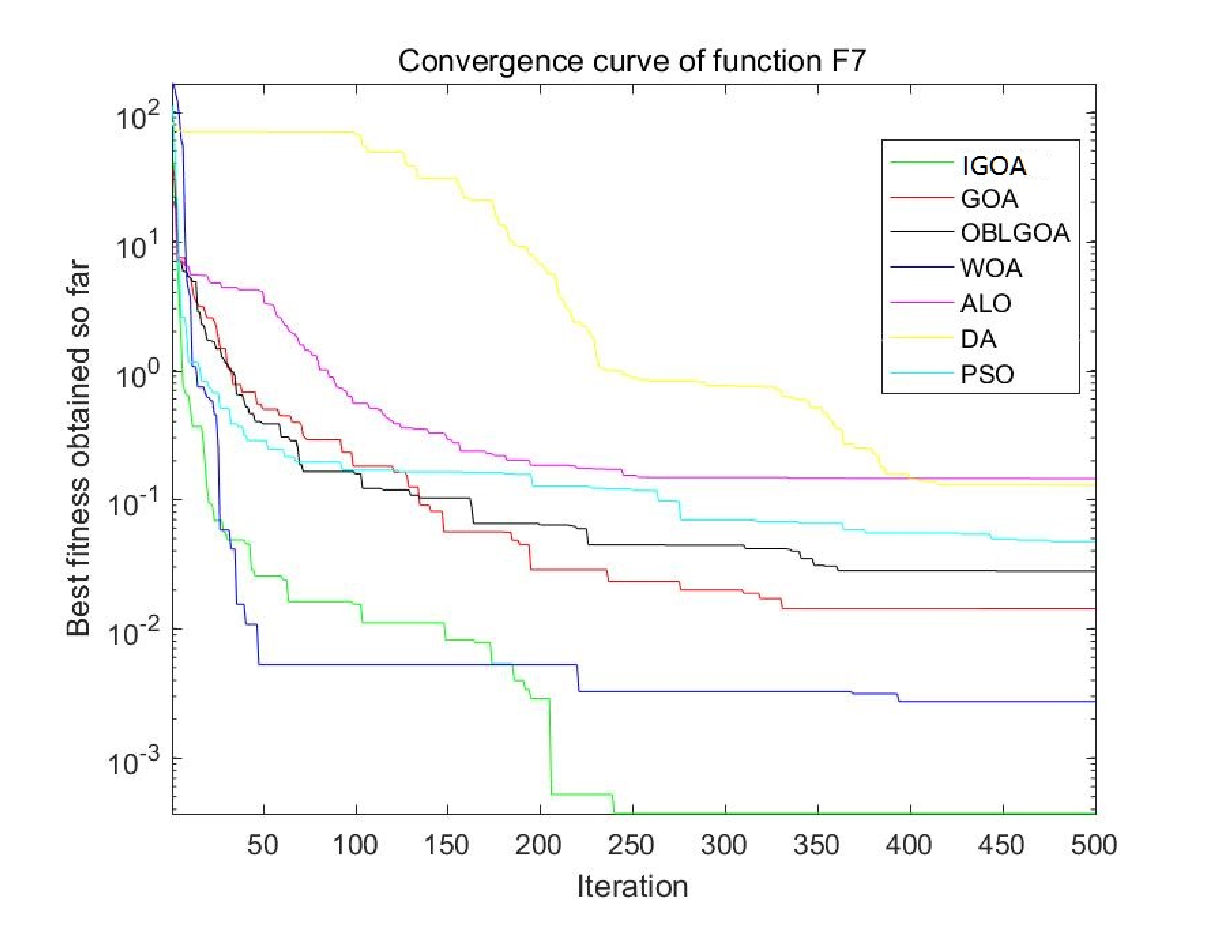
\includegraphics[width=.33\linewidth]{function_F7.eps}\hfill\\[0.5cm]
    % 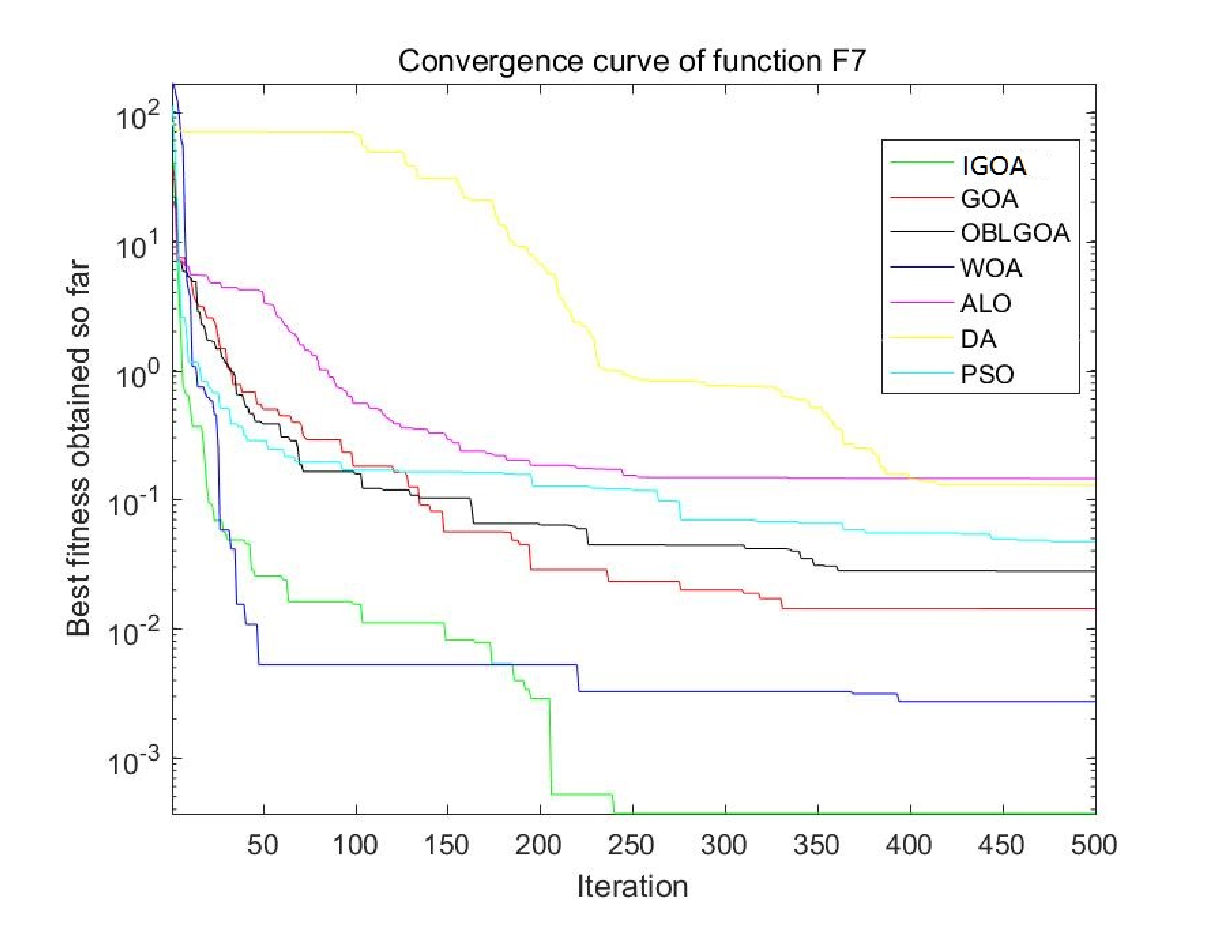
\includegraphics[width=.25\linewidth]{function_F7.eps}\\[0.5cm]
    \centering
    % \includegraphics[width=.25\linewidth]{function_F12.eps}\hfill
    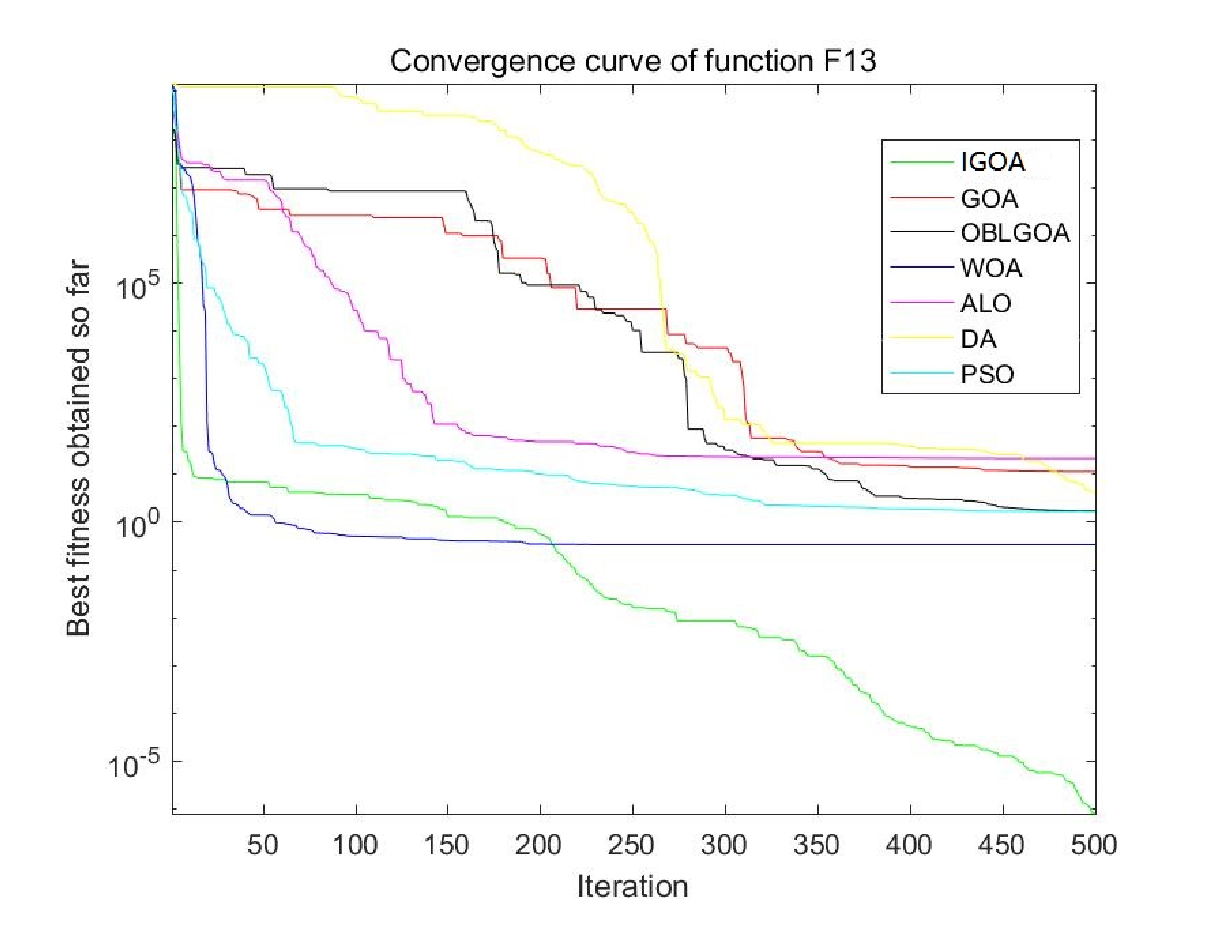
\includegraphics[width=.33\linewidth]{function_F13.eps}\hfill
    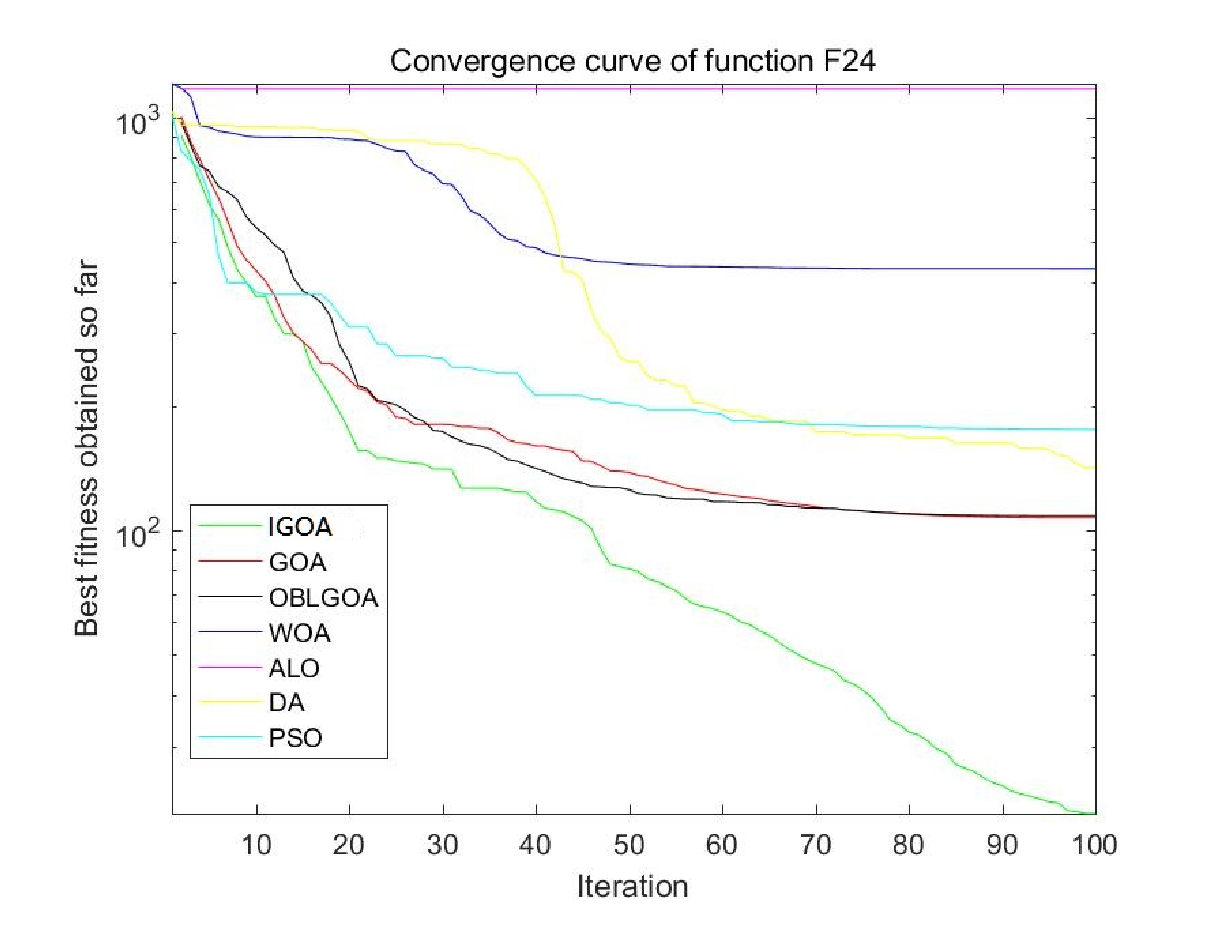
\includegraphics[width=.33\linewidth]{function_F24.eps}
    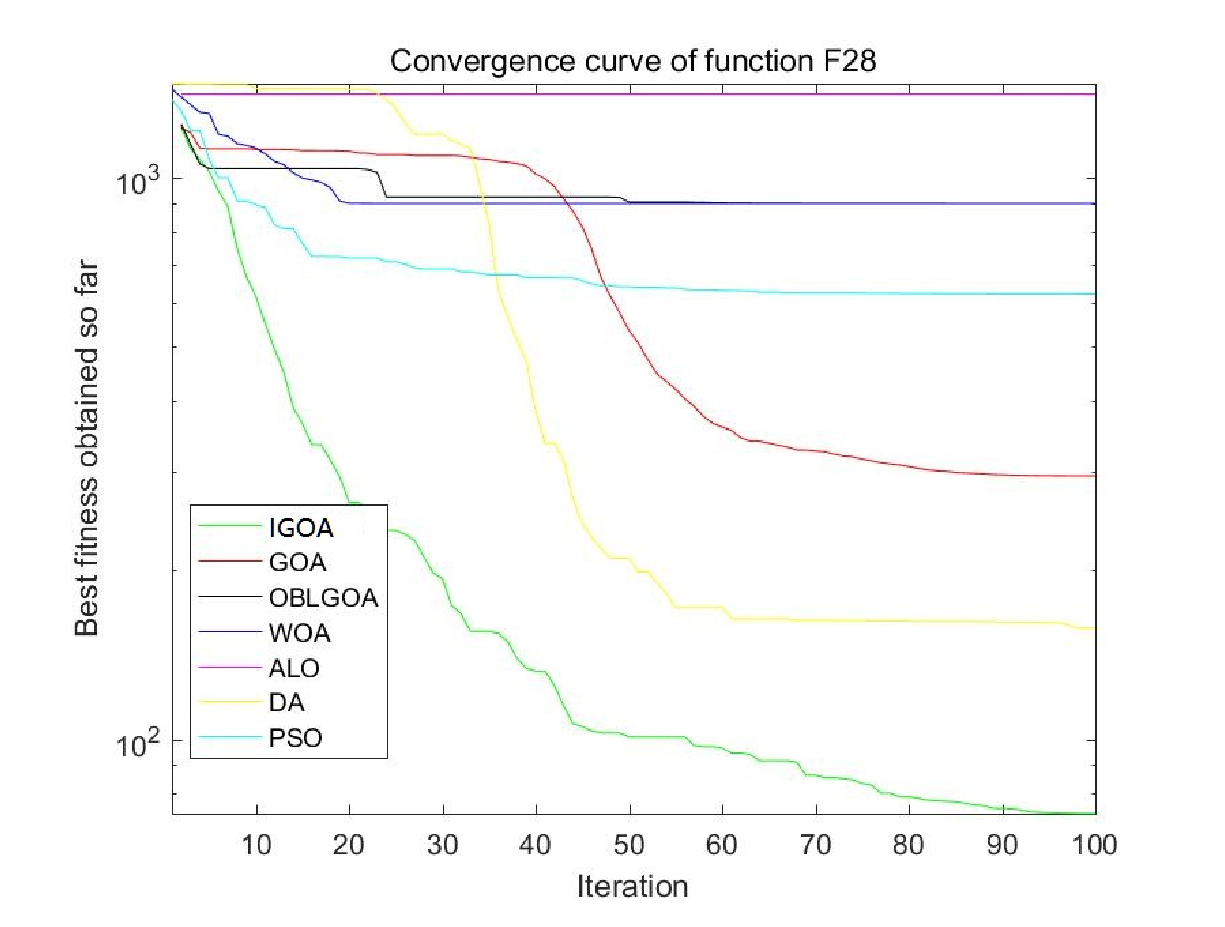
\includegraphics[width=.33\linewidth]{function_F28.eps}\hfill\hfill\\[0.5cm]
    % \includegraphics[width=.25\linewidth]{function_F15.eps}\hfill
    % 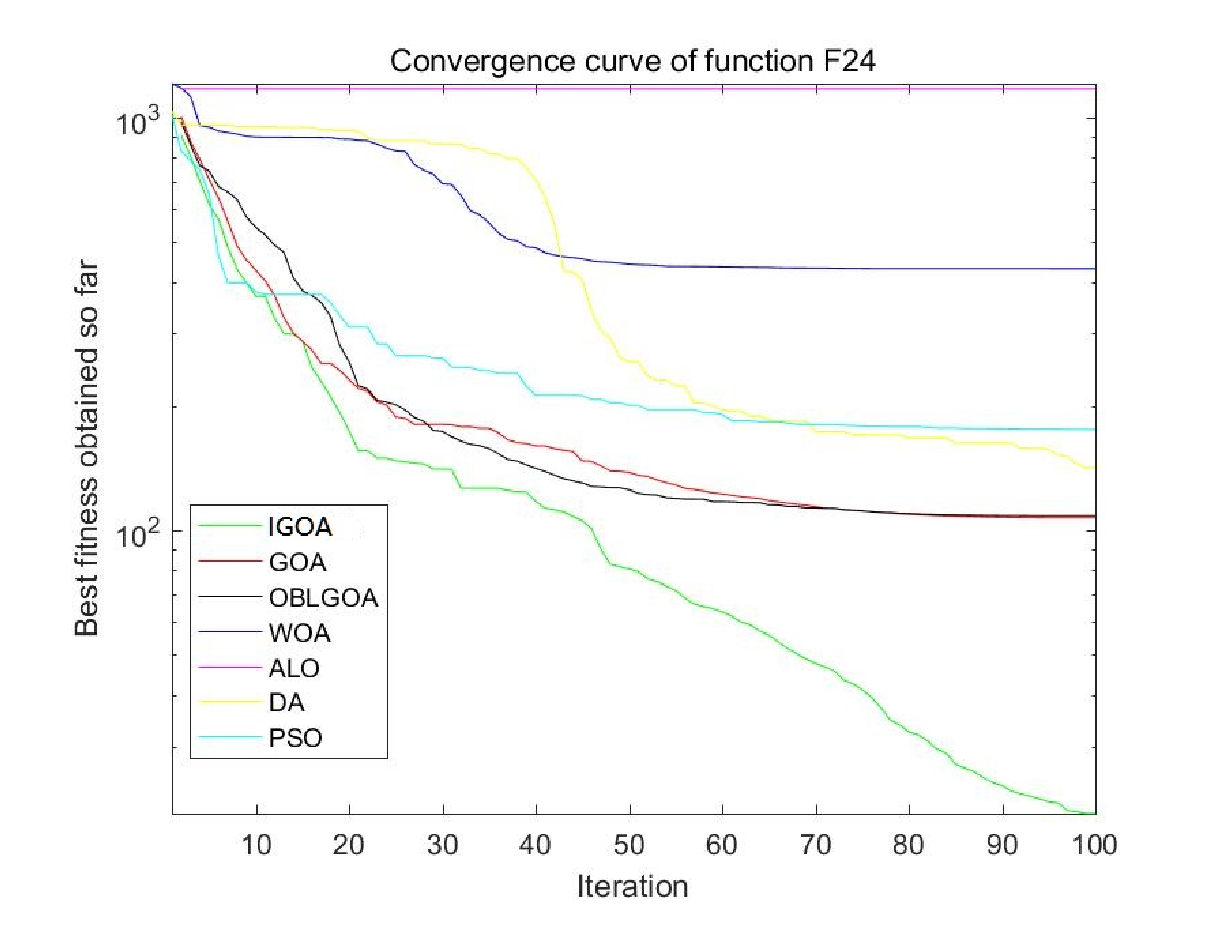
\includegraphics[width=.25\linewidth]{function_F24.eps}\\[0.5cm]
    % \centering
    % \includegraphics[width=.25\linewidth]{function_F25.eps}\hfill
    % \includegraphics[width=.25\linewidth]{function_F26.eps}\hfill
    % 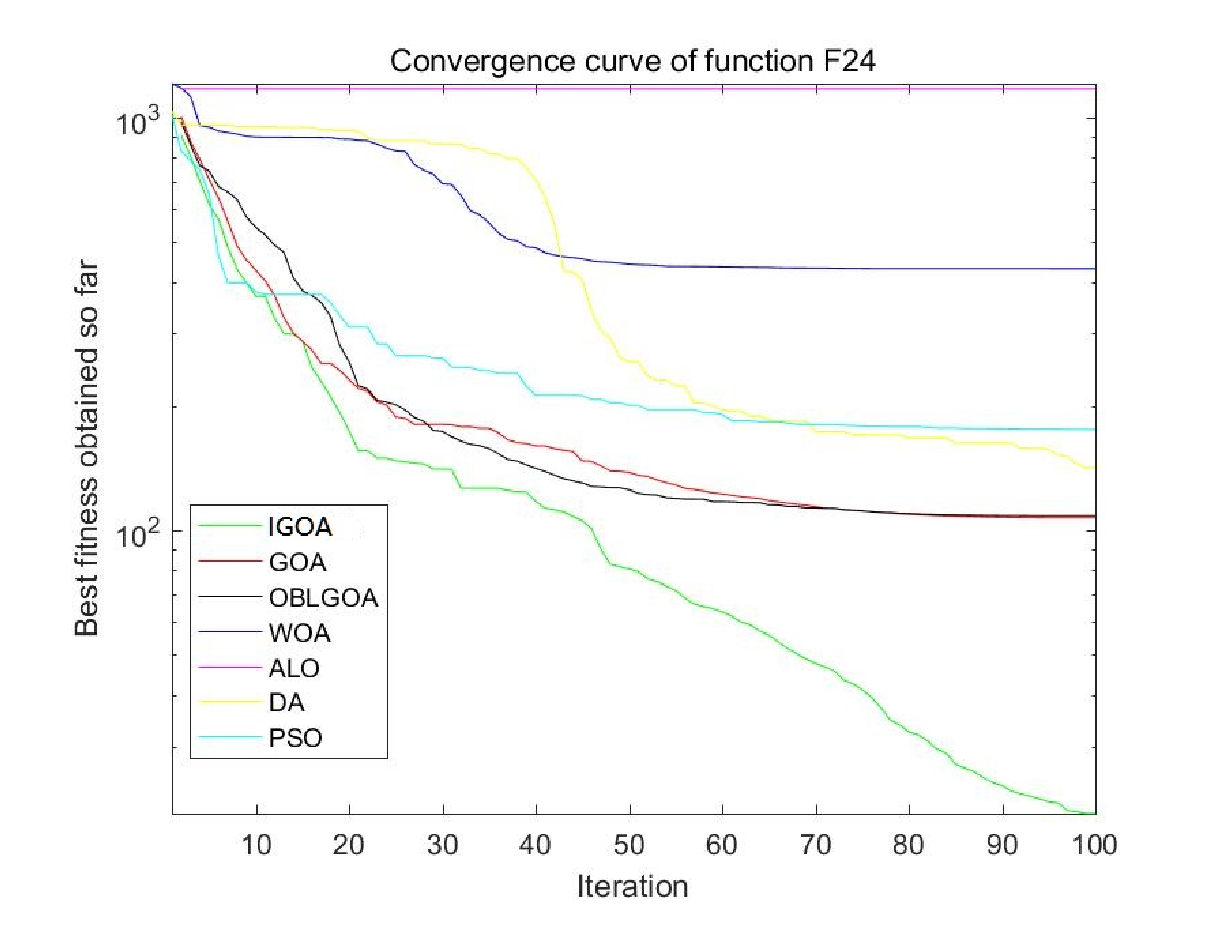
\includegraphics[width=.5\linewidth]{function_F24.eps}\hfill
    % 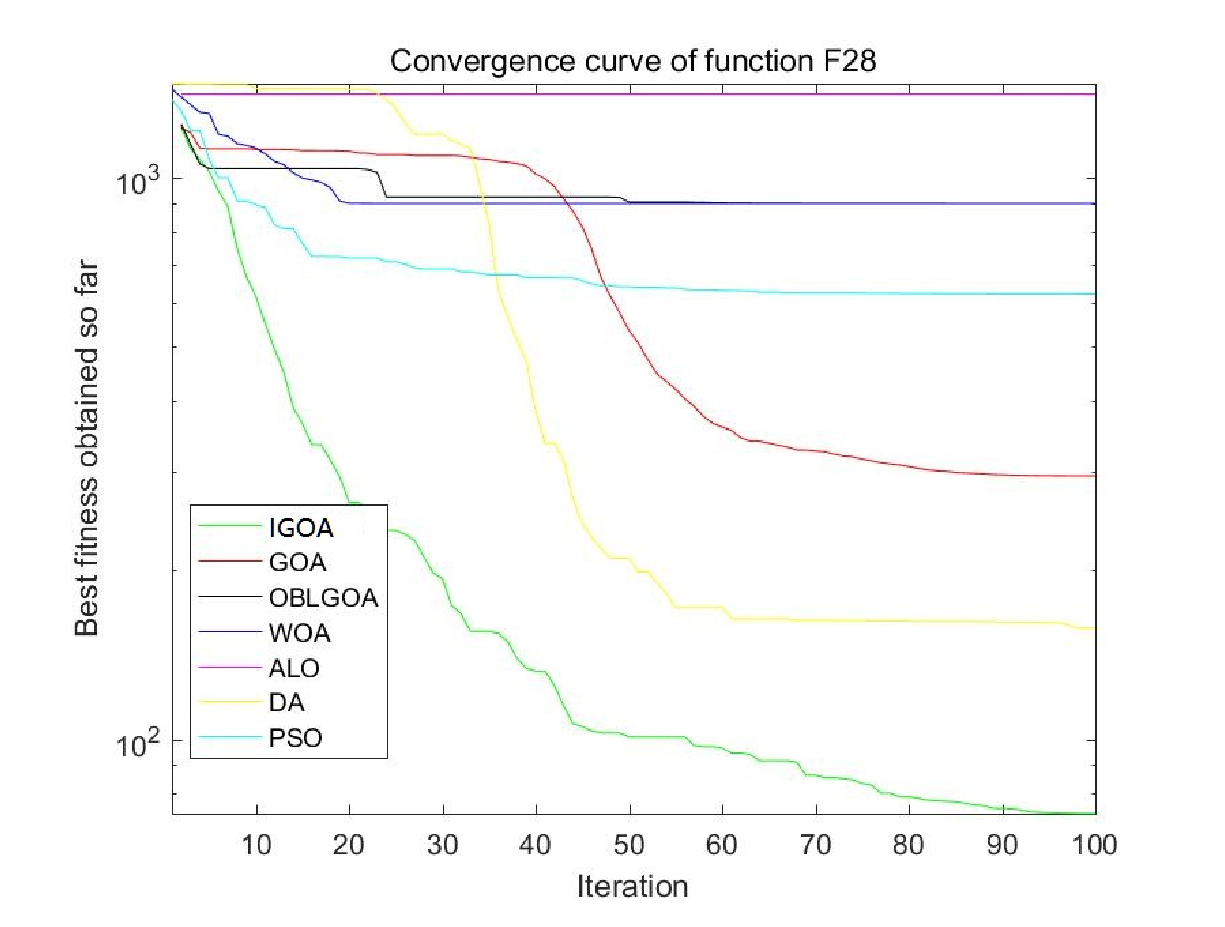
\includegraphics[width=.5\linewidth]{function_F28.eps}\hfill\\[0.5cm]
    % \includegraphics[width=.25\linewidth]{function_F29.eps}\\[0.5cm]
  \caption{Convergence curves for all the 7 algorithms over some benchmark functions }
  \end{figure}


水平轴是当前迭代的数量,垂直轴是迄今为止获得的最佳适应值。为了使曲线更加可区分,在垂直轴上使用对数。 \ emph {图2}中的曲线图像表明,在大多数搜索过程中,IGOA可以相对于整个搜索过程保持较大的斜率。这种现象可能意味着所提出的非线性舒适区参数可以有助于充分利用每次迭代。曲线跨度在大多数函数中都是充足的,这可以表明基于$ L \ acute {e} vy $ flight的局部搜索机制使算法更具创造性。曲线突然出现在\ emph {F3},\ emph {F4},\ emph {F7}中,\ emph {F28}表明随机跳跃策略可以帮助搜索跳出局部最优。收敛曲线表明,所提出的IGOA可以使搜索过程比其他人更快地收敛。

% The convergences rate of the algorithms are discussed in this part. The convergence curves of IGOA and all the other 6 algorithms for comparison over part of the benchmark functions are shown in \emph{Figure 2}. The horizontal axis is the number of the current iteration, and the vertical axis is the best fitness value obtained so far. To make the curve more distinguishable, the logarithm is used in the vertical axis. The curve image in \emph{Figure 2} indicates that IGOA can keep a large slope relatively for the entire search process in most of the search processes. This phenomenon can mean that the proposed nonlinear comfort zone parameter can contribute to making full utilization of every iteration. The curve span is ample in most of the functions, which can suggest that the local search mechanism based on $L\acute{e}vy$ flight makes the algorithm more creative. Some sudden drops of the curve occurred frequently in \emph{F3}, \emph{F4},\emph{F7}, and \emph{F28} show that the random jumping strategy can help the search jump out of the local optimum. The convergence curves demonstrate that the proposed IGOA can make the search process converge more rapidly than others generally.
\section{任务调度问题}\label{sec:task_scheduling_problems}
\subsection{问题描述}

任务调度问题是云计算领域中常见的问题\ cite {qiao2016an},edge computing area \ cite {guo2017energy}和SEA Service System \ cite {wang2015research}。 大量用户会产生大量任务。 因此,当大量用户同时询问服务时,系统应该有效地处理任务,这可能是计算系统的基本问题,尤其是在资源受限的条件下。 在任务调度问题中,到达调度中心的一系列任务等待分配给特定的执行节点。
% Task scheduling problem is a common problem in cloud computing area\cite{qiao2016an}, edge computing area\cite{guo2017energy} and SEA Service System\cite{wang2015research}. Massive users produce massive tasks. Thus the system should handle the tasks efficiently when a large number of users ask the service at the same time, which can be an essential problem of the computing system, especially in resources constrained conditions. In task scheduling problems, a series of tasks arriving at the scheduling center wait to be allocated to a particular execution node. 

由于资源条件,工作负载,处理速度和任务类型的不同,执行节点在此问题中可能是异构的。 任务调度的不同解决方案可能导致不同的后果,并且优秀的解决方案可能会影响很多。 对于服务提供商,将任务分配给适当的节点可以节省能源并减少预算。 对于服务使用者,将任务调度到高效节点可以减少等待时间并改善用户体验。
% The execution node might be heterogeneous in this problem because of the difference in the resource condition, workload, processing speed and the type of task. A different solution to task scheduling could lead to different consequence, and an excellent solution can affect a lot. For service providers, allocating a task to the proper node can save energy and reduce the budget. For service consumers, scheduling the task to the efficient node can decrease the waiting time and improve the user experience. 

任务调度问题可能是一个优化问题,它是一个NP难问题\ cite{tawfeek2013cloud}。应用了许多算法来解决任务调度问题。一些基于最佳资源选择(BRS)的算法,如Max-Min,Min-Min和Sufferage,是解决任务调度问题的传统方法\ cite {qiao2016an}。当任务数量增加时,任务的维度也会增加,这会扩大搜索空间并使优化问题更加复杂。传统算法无法处理这种情况。近年来,许多元启发式算法被应用于解决任务调度问题。 Goldberg在1988年提出的遗传算法(GA)是一种着名的进化算法,它代表了一种解决任务调度问题的染色体调度方案。由于交叉和变异的操作,GA计算起来很复杂。粒子群算法(PSO)是Kennedy和Eberhard在1995年提出的经典元启发式算法.PSO将调度解决方案表示为离散粒子,并通过群体的个人最佳和全局最佳信息进行演化。 PSO很容易陷入局部最优,并且在处理多模态问题时表现不佳。
% Task scheduling problem can be an optimization problem, and it is an NP-hard problem\cite{tawfeek2013cloud}. Many algorithms are applied to solve the task scheduling problem. Some algorithms based on best resource selection(BRS) such as Max-Min, Min-Min, and Sufferage are traditional methods to solve task scheduling problems\cite{qiao2016an}. The dimension of the tasks can also increase when the number of tasks increases, which can enlarge the search space and make the optimization problem more complicated. The traditional algorithms could not handle this situation. In recent years many meta-heuristic algorithms were applied to solve the task scheduling problem. Genetic algorithm(GA) proposed by Goldberg in 1988 is a famous evolutionary algorithm, and it represents a scheduling scheme as a chromosome to solve the task scheduling problem. GA is complicated to calculate because of its operations of crossover and mutation. Particle Swarm Algorithm (PSO) is a classical meta-heuristic algorithm proposed by Kennedy and Eberhard in 1995. PSO represents a scheduling solution as a discrete particle and evolves by the information of the personal best and the global best of the swarm. PSO is easy to fall into local optimum, and it does not perform well when dealing with multimodal problems. 

最近提出了一些元启发式算法,如DA,WOA,GOA等。 在这项工作中,建议的IGOA用于任务调度问题。 将调度到M个节点的N个任务的解决方案抽象为表示搜索空间中的位置的N维离散矢量。 每个解决方案可以对应于系统的完工时间和预算,并且可以使用完工时间和预算来计算适合度值。 一些搜索代理通过IGOA的搜索策略在整个搜索空间中搜索最佳适应度。
% Some recently proposed meta-heuristic algorithms are used such as DA, WOA, GOA and so on. In this work, the proposed IGOA is employed for task scheduling problems. A solution of N tasks scheduled to M nodes is abstracted as an N-dimension discrete vector which represents a position in the search space. Each solution can correspond to a makespan and a budget of the system, and a fitness value can be calculated with the makespan and budget. Several search agents search in the whole search space for the best fitness by the search strategy of IGOA.

\subsection{任务调度模型}
在本文中,我们假设用户启动\ emph {N}任务,这些任务是$ {T_1,T_2,... T_N} $和\ emph {M}个节点,$ \ {S_1,S_2,... S_M \ } $正在等待处理它们。 任务调度模型描述如下。
% In this paper, we assume that users start \emph{N} tasks which are ${T_1,T_2,...T_N}$ and \emph{M} nodes which are $\{S_1,S_2,...S_M\}$ are waiting to handle them. The task scheduling model is described as follows.
\begin{enumerate}[]
    \item The set of \emph{N} tasks is $\{T_1,T_2,...T_N\}$, and $T_i$ represents the resource that the \emph{i-th} task consumes.
    \item The set of \emph{M} nodes is $\{S_1,S_2,...S_M\}$ and $S_j$ represents the maximum amount of resources that the \emph{j-th} node can provide.
    \item A task can be operated at any node as long as the node can provide enough resource, which means $T_i \leq S_j$.
    \item Every node can handle only one task at the same time. Multiple tasks can be run sequentially on the same node. 
    \item There are K types of all the tasks. The vector of types of tasks is $tot[N]$, and $tot_i$ which is an integral value in [1, K] represents the type of \emph{i-th} task.
    \item The ability of every node to handle different type of task is different. The matrix of operating speed is $mips[M,K]$. $mips_{j}^{k}$ represents the resource that the type \emph{k} task can consume on the \emph{j-th} node in a unit time. The working time for the \emph{i-th} task running on the \emph{j-th} node which is $et_{ij}$ is calculated as follows.
    \begin{eqnarray}
        et_{ij}= \begin{cases}
            \frac{T_i}{mips_{j}^{tot_i}} & task\  i\  runs\  on\  node\  j \\
            0&task\  i\  does\  not\  runs\  on\  node\  j 
            \end{cases} 
    \end{eqnarray}
    \item The makespan of the \emph{j-th} node which is $st_j$ is calculated by adding all the operating time of the tasks handled on the \emph{j-th} node. The equation is shown as follows.
    \begin{eqnarray}
        st_{j}=\sum_{i=1}^{N} et_{ij}
    \end{eqnarray}
    The total \emph{Makespan} is the longest time for all the nodes. \emph{Makespan} is calculated as follow.
    \begin{eqnarray}
        Makespan=\max\{st_j | j=1,2,3...M\}
    \end{eqnarray}
    \item The work node can produce the extra budget when it is working. The budget is only related to the time of working, regardless of the type of task running on it. The vector of the price of the nodes is $bps[M]$ which represents the budget that the \emph{j-th} node generate in a unit time.
    \item  The total \emph{Budget} is calculated by adding all the budget of all the nodes. \emph{Budget} is calculated as follows.
    \begin{eqnarray}
        Budget=\sum_{j=1}^{M} (st_j \times bps_j)
    \end{eqnarray}
    \item Makespan and budget can describe the cost of the problems in two aspects. A unified evaluation fitness is required. In this module, the fitness of the problem is defined as the mixture of makespan and budget with weight parameters of $\alpha$ and $\beta$. The \emph{fitness} is calculated as follows.
    \begin{eqnarray}
        fitness=\alpha Makespan + \beta Budget
    \end{eqnarray}
    \item The search process is continuous, but the solution to the problem is discrete. When a step of search is finished, the search agent should adjust itself to the nearest integral location.
    \item The switching time between two tasks on the same node is ignored in this module. The transmission time among the edge nodes is also ignored. 
\end{enumerate}
\subsection{实验结果}
在此任务调度模块中,\emph{N}任务分为\emph{K}类型,\emph{M}工作节点正在准备处理它们。 任务调度模块的参数选择的细节取决于具体问题,这里不再讨论。 在这项工作中,不失一般性,\emph{K},\emph{N}和\emph{M}分别设置为4,10和5。 为了平衡\emph{Makespan}和\emph{Budget}对\emph{fitness}的影响,系数$ \alpha $和$ \beta $设置为0.7和0.3。 上述参数设定如表\ref{tab:resource_and_type_tasks}所示。
% In this task scheduling module, \emph{N} tasks are divided into \emph{K} types, and \emph{M} working nodes are preparing to handle them. The specifics of the parameter selection of the task scheduling module depend on the specific problem and will not be discussed here. In this work, without loss of generality, \emph{K}, \emph{N} and \emph{M} are set to 4,10 and 5 respectively. To balance the impact of \emph{Makespan} and \emph{Budget} on \emph{fitness}, the coefficients $\alpha$ and $\beta$ are set to 0.7 and 0.3. Those parameters mentioned above are set as follows.
\begin{eqnarray}\label{eqn:K_N_M}
    K=4;\ N=10;\ M=5;\ \alpha=0.7;\ \beta=0.3; 
\end{eqnarray}
The vector T, tot, S and bps, and the matrix mips are set as \emph{Table 10-12}.
\begin{table}[!htbp]
    \centering
    \caption{Resources and types about tasks}\label{tab:resource_type_tasks}
    \renewcommand\arraystretch{1.3} 
    % \scriptsize
\begin{tabular}{*{11}{c}}
    \hline
   task& 1& 2& 3& 4& 5& 6& 7& 8& 9& 10\\
    \hline
   T & 40& 20& 30& 40& 25& 35& 45& 10& 5& 10 \\
    \hline
   tot &1& 1& 1& 2& 2& 2& 3& 3& 4& 4 \\
    \hline
   
   \end{tabular}
\end{table}

\begin{table}[!htbp]
    \centering
    \caption{Resource and bps about nodes}\label{tab:resource_bps_nodes_tasks}
    \renewcommand\arraystretch{1.3} 
    % \scriptsize
\begin{tabular}{*{6}{c}}
    \hline
   node& 1& 2& 3& 4& 5\\
    \hline
   S & 100& 50& 150& 100& 80 \\
    \hline
   bps &0.5& 0.2& 0.8& 0.1& 0.5 \\
    \hline
   
   \end{tabular}
\end{table}

\begin{table}[!htbp]
    \centering
    \caption{Mips about tasks and nodes}\label{tab:mips_tasks_nodes}
    \renewcommand\arraystretch{1.3} 
    \begin{tabular}{|c|c|c|c|c|c|}
        \hline
        
        {{$mips_j^k$} }& \multicolumn{4}{|c|}{k:1-4} \\
        
        \hline
        \multirow{5}*{j:1-5}&5& 2& 10& 8\\
        \cline{2-5}
        &2& 4& 2& 1\\
        \cline{2-5}
        &8& 10& 10& 5\\
        \cline{2-5}
        &2& 1& 3& 4\\
        \cline{2-5}
        &5& 5& 8& 8\\
        \hline
        \end{tabular}
\end{table}   

在这项工作中,6个算法与提议的IGOA进行了比较。 每种算法使用30个搜索代理。 为了减少意外因素的影响,对每种算法进行了30次测试,并计算并比较了平均值,标准差,最佳值和最差值等统计数据。 实验结果如表\ref{tab:results_task_scheduling}所示。
% In this work, 6 algorithms were compared with the proposed IGOA. 30 search agents were employed in each algorithm. In order to reduce the impact of accidental factors, every algorithm was tested for 30 times and the statistical data such as average value, standard deviation, best value and worst value were calculated and compared. The result of the experiment is listed as \emph{Table 13}. 
\begin{table}[!htbp]
    \centering
    \caption{Results about task scheduling}\label{tab:results_task_scheduling}
    \renewcommand\arraystretch{1.3} 
    % \scriptsize
\begin{tabular}{*{6}{c}}
    \hline
    algorithm&average&std&best&worst&promotion\\
    \hline
    IGOA& 13.50&	0.62&	12.63&	14.62&	0    \\
    \hline
    GOA & 14.95&	0.82&	13.50&	16.67&	9.7\%    \\
    \hline
    WOA &14.08&	0.75&	13.02&	15.93&	4.1\%    \\
    \hline
    ALO &19.83&	2.89&	16.02&	26.76&	31.9\%    \\
    \hline
    DA &19.00&	2.49&	15.62&	26.81&	29.0\%    \\
    \hline
    PSO &17.93&	1.68&	13.96&	22.29&	24.7\%\\
    \hline
    OBLGOA &14.85&	0.74&	13.30&	16.27&	9.1\%\\
    \hline
   
   \end{tabular}
\end{table}

实验结果表明,所提出的IGOA在所有领域都优于其他算法。 IGOA在平均值方面可以做得最好,对于最小的标准偏差它可以更稳定。 它可以找到所有算法的最佳解决方案,并且可以控制它可以找到的最差值。 与其他算法相比,IGOA可以将平均值分别提升9.7%,4.1%,31.9%,29.0%,24.7%和9.1%。
% The result of the experiment demonstrated that the proposed IGOA outperformed the other algorithms in all field. IGOA can do best in average values, and it can be more stable for the smallest standard deviation. It can have the ability to find the best solution over all the algorithms, and it can control the worst value which it can find. Compared with the other algorithms, IGOA can promote the average values respectively by 9.7\%, 4.1\%, 31.9\%, 29.0\%, 24.7\%, and 9.1\%.

\section{本章小结}\label{sec:task_scheduling_summary}